% Compile with the XeLaTeX engine (on Overleaf: Menu -> Compiler -> XeLaTeX).
%\documentclass[11pt,a4paper]{article}
%\documentclass[a4paper,fleqn]{cas-sc}
%\documentclass[a4paper,fleqn]{cas-dc}
%\usepackage[authoryear]{natbib}
%\usepackage{fontspec}
%\setmainfont{Latin Modern Roman}
%\setsansfont{Latin Modern Sans}
%\setmonofont{Latin Modern Mono}
%\usepackage{fontspec}
%\setmainfont{DejaVu Serif}[Scale=0.92]
%\setmonofont{DejaVu Sans Mono}[Scale=0.82]
%\usepackage{polyglossia}
%\setmainlanguage{english}
%\setotherlanguage{russian}
%\usepackage[a4paper,margin=2.5cm]{geometry}
%\usepackage{amsmath,amssymb}
%\usepackage{booktabs}
%\usepackage[font=footnotesize,labelfont=bf]{caption}  % smaller font for figure/table captions
%\usepackage{tabularx}
%\newcolumntype{L}{>{\raggedright\arraybackslash}X}
%\usepackage{graphicx}
%\usepackage{microtype}
%\usepackage[numbers,sort&compress]{natbib}
%\usepackage[hidelinks]{hyperref}
%\usepackage{xurl}  % break long URLs across lines
% Layout settings: suppress overfull lines without loose justification.
%\graphicspath{{figures/}}
%\tolerance=1400
%\emergencystretch=2.5em
%\hbadness=2200
%\frenchspacing


%% 
%% Copyright 2019-2021 Elsevier Ltd
%% 
%% This file is part of the 'CAS Bundle'.
%% --------------------------------------
%% 
%% It may be distributed under the conditions of the LaTeX Project Public
%% License, either version 1.2 of this license or (at your option) any
%% later version.  The latest version of this license is in
%%    http://www.latex-project.org/lppl.txt
%% and version 1.2 or later is part of all distributions of LaTeX
%% version 1999/12/01 or later.
%% 
%% The list of all files belonging to the 'CAS Bundle' is
%% given in the file `manifest.txt'.
%% 
%% Template article for cas-sc documentclass for 
%% single column output.

\documentclass[a4paper,fleqn]{cas-sc}

% If the frontmatter runs over more than one page
% use the longmktitle option.

%\documentclass[a4paper,fleqn,longmktitle]{cas-sc}

% \usepackage[numbers]{natbib}
\usepackage[authoryear]{natbib}
% \usepackage[authoryear,longnamesfirst]{natbib}

\usepackage{subcaption}
\usepackage{tabularx}
\usepackage{graphicx}
\graphicspath{{figures/}}
\usepackage{xcolor, soul}
% cas-common.sty defines L as a non-wrapping fill column; the feature tables need a wrapping one.
\newcolumntype{L}{>{\raggedright\arraybackslash}X}

%%%Author macros
\def\tsc#1{\csdef{#1}{\textsc{\lowercase{#1}}\xspace}}
\tsc{WGM}
\tsc{QE}
%%%

% Uncomment and use as if needed
%\newtheorem{theorem}{Theorem}
%\newtheorem{lemma}[theorem]{Lemma}
%\newdefinition{rmk}{Remark}
%\newproof{pf}{Proof}
%\newproof{pot}{Proof of Theorem \ref{thm}}

\begin{document}
\let\WriteBookmarks\relax
\def\floatpagepagefraction{1}
\def\textpagefraction{.001}


\shorttitle{Integrated World Model}    

\title[mode = title]{An Integrated World Model for Strategic Planning and Scenario Analysis}
\author[1]{Nazar S.~Sotiriadi}
\cormark[1]
\ead{sotiriadi.n.s@gmail.com}
\author[1,2]{Andrei A. Osiptsov}[]
\affiliation[1]{organization={JSC Sberbank of Russia}, addressline={Kutuzovsky avenue, 32}, city={Moscow}, citysep={}, postcode = {121170}, country={Russian Federation}}
\affiliation[2]{organization={Skolkovo Institute of Science and Technology (Skoltech)}, addressline={Bolshoy Boulevard 30, bld. 1}, city={Moscow}, citysep={}, postcode = {121205}, country={Russian Federation}}

\date{\today}

%\begin{document}
\maketitle

\begin{abstract}
\noindent
This paper describes an integrated simulation model of the world, in which the economy, climate
and carbon cycle, warming damages, natural resources, society and politics, interstate
relations, culture, crisis and finance mechanisms are coupled within a single computational
loop. The model is organized as a system of interacting countries and includes 57 country agents and regional aggregates. Simulation advances year by year: each block updates its state annually, and the results are passed to the next year and to adjacent blocks. The aim is not to deliver a point forecast of the future but to provide a tool for strategic planning and scenario analysis: playing out coherent development scenarios, comparing alternative policy decisions, quantifying uncertainty through ensembles, and detecting weak signals of approaching structural shifts -- including for the management of systemic risks. We set out the problem and the model's place among existing approaches, its architecture and the mathematics and empirical basis underlying each block, the calibration and validation procedure with the resulting metrics, sensitivity analysis and ensemble uncertainty quantification, an explicit list of limitations, and typical use cases, including a decision-game layer built on the same core whose automated playthrough distributions double as a stress test of the coupled dynamics. The economic and climate blocks are calibrated on historical data and evaluated retrospectively, including a temporal hold-out test in which parameters constrained on data through 2019 are scored out-of-sample on 2020--2023. The society, politics, and geopolitics blocks are assessed against a more modest criterion -- improvement over naive benchmarks (persistence, linear extrapolation, and base-rate forecasts).

\medskip
\noindent\textbf{Keywords:} integrated assessment model (IAM), strategic planning, scenario analysis, uncertainty quantification, risk management, weak signals.
\end{abstract}


\section{Introduction}


Strategic planning and scenario analysis over long horizons --- from government policy to
corporate strategy --- require a tool, in which climatic, economic, and socio-political processes
are considered jointly rather than in isolation; the same need arises in the management of
systemic risks. In practice, an analyst must rely on a patchwork of disparate models: climate
models describe atmospheric physics but contain almost no finance or politics; integrated
assessment models (for example, the DICE, RICE, and FUND families) couple the economy and climate
but typically lack sovereign finance, interstate relations, and social dynamics \citep{nordhaus2017}; macroeconomic models describe the monetary sphere in detail but ignore natural capital. As a result, the mutual influence of these domains -- for example, the path from warming to falling crop yields, rising prices, social tension, and on to political instability and conflict -- falls outside the scope of any single model.

Yet it is precisely the coupling of these channels that determines how long-run development
scenarios unfold and where systemic risks accumulate. The absence of a coherent model spanning
climate, the economy, society, and geopolitics at once is a substantive gap, felt in strategic
planning and risk management alike, where the task is not to assess an isolated shock but to trace
its propagation across interconnected subsystems and to compare alternative development
trajectories. This paper describes a model built to fill that gap. We emphasize a principled stance
from the outset: the model does not claim to be an infallible predictor. Assessments of multi-year
forecasts show that even professional growth forecasts at horizons of two to five years often fail
to beat a naive extrapolation of the mean \citep{celasun2021}. {\it A realistic goal therefore is not
in point forecast but in the ability to reproduce scenarios coherently, with proper tracking of the measure of uncertainty along each scenario.}

The novelty of this work lies not in any single block but in the integration and the breadth of
coupling; stated exactly: (i)~a single annual loop that carries the state through the economy,
climate, resources, society, politics, and interstate relations \emph{including discrete crises},
where every listed comparator stops at two or three of these domains; (ii)~uncertainty
quantification (ensembles, history matching) built into the workflow rather than added post hoc;
and (iii)~an optional strategy layer in which large-language-model agents set country policies
while all consequences are computed by the deterministic core. The crisis module and the
language-model layer are components of this integration, not the novelty claim by themselves. Integrated assessment models (IAM) such as DICE and FUND and large modeling frameworks (GCAM, MESSAGEix, REMIND) couple the economy and climate in detail but contain no sovereign finance, interstate relations, or
socio-political dynamics; the classic world-system models (World3) lack an explicit price economy
and a modern-grade climate. The distinguishing feature of the proposed model -- the Global
Integrated Model (GIM) -- is that it carries the loop through to society, geopolitics, and discrete
crises, and embeds large-language-model agents that play as countries
(Table~\ref{tab:compare}, Section~\ref{sec:repo}); a controlled benchmark that quantifies this
advantage against sectoral models is given in Appendix~\ref{app:benchmark}.

\begin{table*}[t]
\centering
\caption{Feature comparison with representative integrated, energy-economy, and world-system
models. Each cell states the specific capability rather than a checkmark; the last column lists
the domains that fall outside each model's scope but inside the scope of the question this paper
addresses (shock propagation across economy, climate, society, and geopolitics).}
\label{tab:compare}
\small
\begin{tabularx}{\linewidth}{@{}l L L l L@{}}
\toprule
Model & Paradigm & Domains covered & Spatial units & Not represented \\
\midrule
DICE\,/\,RICE & welfare optimisation & climate + aggregate economy, quadratic damages & world (RICE: 12 regions) & prices, finance, resources, society, politics, conflict, discrete crises \\
GCAM & recursive-dynamic market equilibrium & energy--land--water--climate detail & 32 regions & sovereign finance, social and political dynamics, interstate conflict \\
MESSAGEix & energy-system optimisation (+MACRO) & energy technology detail, land use, climate & 11+ regions & society, politics, geopolitics; crises only as scenario inputs \\
E3ME & econometric simulation \citep{mercure2018} & energy--economy--environment, demand-led macro & $\sim$70 regions & interstate relations, conflict, endogenous discrete crises \\
T21\,/\,iSDG & system dynamics \citep{barney2002} & country-level economy--society--environment (SDG scope) & one country per model & interstate trade network, geopolitics, multi-country shock propagation \\
World3 & system dynamics \citep{meadows1972} & global stocks: population, capital, resources, pollution & global aggregates & price economy, countries, modern climate module, politics \\
GIM (this paper) & recursive simulation of interacting country agents & economy and prices, climate and carbon, resources, society and politics, geopolitics and conflict, discrete crises and stock-flow-consistent finance & 57 country agents & sectoral energy technology detail, optimal-policy search (see text) \\
\bottomrule
\end{tabularx}
\end{table*}

The coverage comparison (Table~\ref{tab:compare}) is usefully complemented by a comparison along
\emph{methodological axes}: the listed models address different problems, so a direct
``better--worse'' ranking is inappropriate, and the distinction is better drawn by solution
paradigm, treatment of uncertainty, and object of validation. In terms of \emph{solution paradigm},
the DICE\,/\,RICE\,/\,FUND family and REMIND rest on welfare optimization (finding an optimal policy
trajectory), GCAM and MESSAGEix on a detailed equilibrium of energy and land-use systems, and World3
on the system dynamics of global aggregates, whereas the proposed model is a recursive simulation of
interacting countries with adaptive expectations. This implies a division of strengths: the
assessment models and energy frameworks are \emph{deeper} within their domains (optimal policy,
sectoral energy detail), and the proposed model does not replace but complements them. Its distinction appears along three dimensions at once: {(i)}~breadth of coupling, carrying the single loop through to
society, geopolitics, and discrete crises --- quantified against sectoral models in a controlled
benchmark in Appendix~\ref{app:benchmark}; {(ii)}~uncertainty as a first-class object ---
ensembles and history matching are built into the workflow rather than added post hoc; and
{(iii)}~the testability of non-standard blocks (conflict-risk ranking by AUC, an identified
lagged channel between the economy and society), which comparable models simply do not contain. The
model thus occupies the niche of a tool for broad scenario coverage and shock-propagation analysis,
enabling rather than replacing specialized models within their domains.

\section{The model and its architecture}


\subsection{General design}

The model represents the world as a system of interacting countries evolving year by
year.\footnote{Fifty-seven actors: the 50 largest economies (Taiwan among them) and seven residual
regional aggregates bundling all remaining countries of each region, so that world totals are
conserved. The rationale for the cut at 50 is given with the ensemble results in
Section~\ref{sec:uq}.} The state of
each country comprises economic, resource, social, political, and military variables, as well as
bilateral relations with other countries. Above the countries, the global evolution is governed by macro-variables of climate and the carbon cycle and world resource prices. One model step is one year: blocks update in a fixed order in which the output of one block serves as the input to the next, after which the year's results are passed forward to the following year. The computational core is deterministic;
uncertainty is introduced through ensemble runs with random parameter draws from justified ranges
(Section~\ref{sec:calib}).

Below we describe the model structure decomposed into blocks grouped thematically. For each block, we indicate what it computes, on what mathematics and data it rests, and what it provides to the rest of the model.

\subsection{Economy}


Each country's output is determined by three factors: accumulated capital, employed population,
and consumed energy. The production function is specified as a nested constant-elasticity-of-sub\-sti\-tu\-tion
function (a \emph{capital--labor--energy} form), normalized so that at the calibration base point
it coincides with a Cobb--Douglas production function \citep{arrow1961}:
\begin{equation}
Y = A \, \Theta \, K^{\alpha} L^{\beta} E^{\gamma},
\qquad \alpha = 0.30,\; \beta = 0.60,\; \gamma = 0.042,
\label{eq:prod}
\end{equation}
where $A$ is total factor productivity and $\Theta$ is the technology level. The nested form, with a
capital--energy elasticity of substitution $\sigma_{KE}=0.4$ \citep{vanderwerf2008,koetse2008}, captures how hard it is to substitute
one factor for another: as energy becomes more expensive, the economy shifts toward capital and
reduces energy use.


Equation~\eqref{eq:prod} as written in the Cobb--Douglas limit. The
production core actually computed is the nested form, of which \eqref{eq:prod} is the exact
base-point reduction. Capital and energy form an inner CES composite that is then combined with
labor Cobb--Douglas-style:
\begin{equation}
Y = A\,\Theta\,\Big[\mathrm{KE}_0\big(a_K (K/K_0)^{\rho} + a_E (E/E_0)^{\rho}\big)^{1/\rho}\Big]^{\alpha+\gamma} L^{\beta},
\qquad \rho = \frac{\sigma_{KE}-1}{\sigma_{KE}},
\label{eq:ces}
\end{equation}
with inner weights $a_K = \alpha/(\alpha+\gamma)$, $a_E = \gamma/(\alpha+\gamma)$, base-point
quantities $(K_0, E_0)$ captured per country at the calibration base year, and the normalization
constant $\mathrm{KE}_0 = K_0^{a_K} E_0^{a_E}$. At the base point the bracket equals one, so
\eqref{eq:ces} coincides with the Cobb--Douglas form~\eqref{eq:prod} in level \emph{and} first
derivatives for any $\sigma_{KE}$ --- the normalized-CES discipline that keeps the calibration
point invariant while the substitution behaviour away from it is governed by $\sigma_{KE}=0.4$
(gross complementarity between capital and energy). On the exponent sum: $\alpha+\beta+\gamma =
0.942$ encodes deliberate mild decreasing returns to scale (a proxy for fixed factors and
overhead). Because each country carries a scale factor pinning its base-year output level, the
exponent sum has no compounding level effect: renormalising to constant returns moves 2100 world
product by only $7$--$9\,\%$, a bound enforced by a dedicated regression test, so no hidden
$5.8\,\%$ drag accumulates.


This very mechanism allows a carbon price to restructure the economy
realistically. Capital accumulates by the standard rule
\begin{equation}
K_{t+1} = (1-\delta)\,K_t + s\,Y_t, \qquad \delta = 0.05,
\label{eq:capital}
\end{equation}

where the savings rate $s\thickapprox 0.24$ is modulated by social stability and tension --- the precautionary-saving response to uncertainty \citep{mody2012}. Productivity $A$ grows at a baseline rate of about one percent per year, responding additionally to research
spending, technology diffusion through trade, and a conditional-convergence term in which poorer economies catch up faster --- its slope was fit within the present model to the 2015--2023 cross-section of real purchasing-power-parity output to yield $0.0093$ per log unit of the per-capita output gap to the frontier, so the model reproduces the observed catch-up growth of China and India. For forward projections the drift is anchored to the SSP2 socio-economic development scenario \citep{riahi2017}. The energy, resource, and capital markets clear through prices: energy demand and investment respond to the price of energy and the cost of capital with calibrated elasticities.
Inflation (a Phillips curve with energy cost pass-through), unemployment (Okun's law), the
central-bank rate (a Taylor rule, \citep{taylor1993}), the government budget and debt, and trade
flows are tracked separately. Inflation additionally carries a weak quantity-theory term: excess
growth of broad money (the endogenous stock of bank deposits) above a stable-velocity reference is
passed through to prices, with a pass-through coefficient ($\lambda\thickapprox0.027$) estimated from a
cross-country panel that is small by construction --- consistent with the flat post-1990 Phillips
curve --- and whose estimation independently confirms the model's inflation-persistence anchor. The
economic block reproduces the last decade of actual history and is
therefore not speculative but empirically anchored.

Three boundary clarifications are due here. \emph{Technological change} enters through four
channels: the baseline productivity drift, an R\&D-stock mechanism \`a la Jones fed by research
spending \citep{jones1995}, technology diffusion embedded in trade intensity (importers absorb
productivity from more advanced partners), and the structural decarbonisation of the emission
intensity of output, calibrated on the observed 2015--2023 per-country decline. An explicit
endogenous learning curve for renewable-energy costs (a Wright-law module) is \emph{not} part of
the present core: the aggregate resource block does not resolve individual energy technologies,
and the falling cost of clean energy is carried implicitly by the calibrated decarbonisation
rate. This is an acknowledged simplification relative to energy-system models (GCAM, MESSAGEix),
which resolve it explicitly --- and one reason we position the model as complementing rather than
replacing them. \emph{Demography} is exogenous in the headline run (observed base-year population
with scenario growth rates); a logistic demographic-transition module linking fertility decline to
development is implemented and calibrated but switched off by default, following the same
golden-preservation discipline as other optional mechanisms; migration responds to income gaps and
instability through a gravity specification whose elasticities are anchored to the migration
literature (Section~\ref{sec:limits}). A dedicated \emph{pandemic} submodel does not exist:
epidemic shocks belong to the extreme-event class (discrete shocks to output, trade, and
mortality) rather than to an epidemiological compartment model, so pandemic scenarios are
exercised as exogenous stress tests, not endogenous forecasts.\footnote{Calibration sources for the economic
block: the Penn World Table (factor shares and total factor productivity); the World Bank's World
Development Indicators (gross product, population, energy use, military spending); the forward
productivity drift is anchored to the SSP2 socio-economic development scenarios (IIASA database). A
full list of variables with dataset versions and references is given in the repository~\citep{theclimateguy2026gim} (described in detail in Section~\ref{sec:repo}).}

%file \texttt{data/external/SOURCES.md} 

\subsection{Climate and the carbon cycle}


Output is accompanied by carbon-dioxide emissions, to which a land-use source is added. The emission
intensity of output declines structurally at a country-specific rate that rises with development ---
richer, post-industrial economies decarbonise faster (renewables and the offshoring of heavy
industry), the mirror image of growth convergence and fit to the 2015--2023 per-country
carbon-intensity decline.

The carbon cycle is the standard IPCC AR6 four-pool impulse-response model
\citep{joos2013}: each year's emission pulse $E_t$ is partitioned into four pools with shares
$a_i$ and lifetimes $\tau_i$,
\begin{equation}
C^{(i)}_{t+1} = C^{(i)}_t e^{-1/\tau_i} + a_i E_t, \qquad
a = (0.217,\ 0.224,\ 0.282,\ 0.276), \quad
\tau = (\infty,\ 394,\ 36.5,\ 4.3)\ \text{yr},
\label{eq:pools}
\end{equation}
so a fifth of every ton emitted is effectively permanent while the rest decays on centennial,
decadal, and interannual timescales. Radiative forcing is logarithmic in the summed atmospheric
stock, $F = 5.35 \ln (C/C_0) + F_{\mathrm{non\text{-}CO_2}}$, where the non-CO$_2$ term follows
the SSP2-4.5 marker pathway forward (a plateau of about $0.73$~W/m$^2$ by 2100, rather than an
unbounded extrapolation). Warming is computed by the standard two-reservoir surface--ocean
heat-balance model \citep{geoffroy2013},
\begin{equation}
C_s \dot T = F - \lambda T - \kappa\,(T - T_d), \qquad
C_d \dot T_d = \kappa\,(T - T_d),
\label{eq:ebm}
\end{equation}
with the feedback parameter $\lambda$ set by the equilibrium climate sensitivity and the heat
capacities and exchange coefficient calibrated within the ranges of \citet{geoffroy2013}. This is
exactly the architecture of the reduced-complexity emulators used in the IPCC assessment (FaIR,
MAGICC; \citealp{smith2018fair,meinshausen2011}), and the block passes the same two-number bar
those emulators are constrained to: equilibrium climate sensitivity $3.0\,^\circ$C (AR6 best
estimate) and a transient climate response of $1.79\,^\circ$C under the idealised $1\,\%$-per-year
CO$_2$ ramp, against the AR6 best estimate of $1.8$ (likely range $1.4$--$2.2$); both checks are
pinned in the test suite.

\emph{Tipping points and carbon feedbacks.} Self-amplifying carbon releases are represented by two
explicit, switchable mechanisms: a proportional temperature-dependent flux into the pools (a
permafrost-like feedback, GtCO$_2$ per degree of warming) and a stochastic abrupt-release channel
whose pulse sizes follow a heavy-tailed distribution. Both are \emph{off} in the headline run:
their magnitudes are deeply uncertain, and turning them on by default would let an unvalidated
mechanism dominate validated dynamics. They are exercised in tail-risk scenarios, where the
carbon-feedback coefficient becomes a live parameter of the sensitivity analysis
(Section~\ref{sec:uq}). The block is calibrated to mainstream scientific assessment: driven by observed emissions from a
pre-industrial spin-up, it tracks the observed temperature and carbon record from 1990 to 2023
with a temperature error of $0.096\,^\circ$C and a best-fit equilibrium sensitivity of
$3.0\,^\circ$C \citep{ipcc_ar6_wg1,friedlingstein2023}.\footnote{Sources for the climate block: the
equilibrium-sensitivity estimate --- the IPCC Sixth Assessment Report (Working Group~I); the global
emissions series --- the Global Carbon Project (Global Carbon Budget) and the Our World in Data
compilation; the surface-temperature series for 1990--2023 --- NOAA\,/\,HadCRUT5.} This is a fast
calibrated approximation, appropriate within a model of the economy and society but not a substitute
for a full Earth-system model.

\subsection{Warming damages and the cost of carbon}


Warming returns to the economy as damage: higher temperature reduces output. A quadratic damage
function reducing the level of output is adopted \citep{nordhaus2017,howard2017},
\begin{equation}
\Omega(T) = 1 - 0.0078\,T^{2},
\label{eq:damage}
\end{equation}
corresponding to losses of $3.1\,\%$, $7.0\,\%$, and $12.5\,\%$ of gross product at warming of $+2$,
$+3$, and $+4\,^\circ$C. This coefficient is anchored to the productivity-corrected central estimate
of the Howard--Sterner meta-analysis (about $7\,\%$ of product at $+3\,^\circ$C) --- roughly three
times higher than in DICE-2016R2 \citep{howard2017,burke2015} --- and the damage multiplier is
normalised to the observed 2023 baseline, so damage accrues only for incremental warming above the
present level (no base-year double-count). A direct cross-model check isolates where our headline
cost of carbon comes from: fed DICE's \emph{own} lower damage coefficient and discounting, the
model's marginal-pulse engine returns about \$15 per ton of carbon dioxide at a multi-century
horizon --- below DICE-2016R2's \$31 per ton. That gap is not an engine artefact but a growth effect: our
empirically calibrated growth core (with development convergence, Section~\ref{sec:calib}) raises
future per-capita consumption faster than DICE's exogenous path, so a richer future discounts its
damages more heavily. The higher headline cost of carbon therefore follows from our higher,
empirically grounded damage function (about three times DICE's), and the sub-DICE value
under DICE's own damages indicates that DICE-2016R2 underestimates damages once realistic growth is
imposed. We are explicit about where this specification sits in the newer damage literature. The empirical
frontier has moved beyond deterministic quadratic \emph{level} damages toward panel-identified,
non-linear responses of economic \emph{growth} to temperature
\citep{burke2015,burke2023}: growth effects compound, so the same warming path implies much larger
long-run losses, and the response is non-monotonic (cold countries can gain temporarily). The
model therefore also implements a Burke-type growth-damage channel --- a temperature-dependent
increment to the productivity growth rate, calibrated to the panel estimates --- as a switchable
mechanism. It is off in the headline run for the same golden-preservation reason as other
contested mechanisms: growth-effect magnitudes remain debated within the discipline, and one
widely cited recent panel estimate was retracted after publication, which counsels against letting
this channel drive headline results; switched on, it raises long-horizon damages and the social
cost of carbon substantially, and it is explored as part of the uncertainty analysis rather than
hidden. The quadratic level function~\eqref{eq:damage}, anchored at the meta-analytic central
estimate, remains the auditable, conservative headline choice. From the damage function, the
social cost of carbon --- the economic damage from emitting one additional ton of carbon dioxide,
a standard reference point for climate policy --- is computed by the marginal-pulse method, with a
FaIR-style pulse injected into the carbon pools of~\eqref{eq:pools}. This quantity depends
substantially on the discounting scheme and on the structure of future growth; results are
reported in Section~\ref{sec:calib}.\footnote{Calibration of the damage function draws on the Howard--Sterner
meta-analysis and the panel estimates of Burke and coauthors; the social-cost-of-carbon reference
points are the estimates of the U.S. Environmental Protection Agency (EPA, 2023) and the RFF-SP
project.}

\subsection{Resources}

For each country, stocks, production, and consumption of energy, food, and metals are tracked; world
prices rise when demand exceeds supply, and this price is passed into inflation and on into the
economy. The resource market clears by price with a calibrated demand elasticity; a slow-adjustment
rule is provided as a fallback. Resources are represented in aggregate rather than as detailed
sectoral energy systems.\footnote{The resource block is specified in aggregate: energy indicators
draw on the World Development Indicators; price elasticities are set from generalized market
estimates rather than a dedicated sectoral dataset.}

\subsection{Society, politics, geopolitics, and culture}


For each country the model tracks trust in government, social tension, income inequality,
institutional legitimacy, and protest pressure. These variables respond to the economy --- rising
inflation and unemployment raise tension and erode trust, and high inequality amplifies this effect
--- and, in turn, affect stability and crisis risk. Each pair of countries is linked by a relation:
trade volume, the presence of an alliance, the level of conflict or tension, a state of war, and
sanctions. Each country's military capability is anchored to observed measures of national power
rather than to arbitrarily assigned values \citep{singer1972}: a four-component CINC-style
capability share (population, energy, gross product, and SIPRI military expenditure, the latter
populated at world build from a committed SIPRI-2023 grounding file). The military-expenditure
component matters empirically: the three-component proxy without it reproduces the cross-country
\emph{levels} of military spending well (correlation ${\approx}0.76$) but is anti-correlated with
the post-2022 militarization \emph{dynamics} (correlation of share changes $-0.115$), so no
combination of population, energy, and output carries the militarization signal. A small set of cultural traits
(chiefly individualism, uncertainty avoidance, long-term orientation, and hierarchy), together with
the character of the political regime, influence economic and social behavior \citep{hofstede2010}.
Unlike the economy and climate, no single authoritative calibration dataset exists for these links;
where possible their priors are tied to the literature and to reproducible numbers
(Section~\ref{sec:uq}), and the remainder is expert-set and assessed against a more modest
criterion (Section~\ref{sec:calib}).\footnote{The socio-political and geopolitical variables are
anchored to recognized indices: income inequality --- the SWIID database and the World Bank Gini
index; legitimacy, governance quality, and political stability --- the Worldwide Governance
Indicators; armed conflicts --- the UCDP/PRIO Armed Conflict Dataset (v.~24.1); military capability
--- a CINC-style composite (Correlates of War methodology) whose military-expenditure component is
populated from the SIPRI military-expenditure database; sanctions --- the Global Sanctions Database (v.~3); cultural traits --- the Hofstede indices. Data available at~\citep{theclimateguy2026gim}. 

%(2023 values, committed as \texttt{data/external/sipri\_milex\_2023.csv}); sanctions --- the Global Sanctions Database (v.~3); cultural traits --- the Hofstede indices. The mapping of each variable to its source is described in \texttt{data/external/SOURCES.md}.
} 

Traits that did not in fact affect outcomes have been removed from the model, so that it does not mimic cultural detail it does not use.

\emph{Operational definition of social tension.} Tension is a latent index on $[0,1]$, but its
construction is fully specified and cross-country comparable. At the base year it is a fixed-weight
composite of observed quantities: $0.35\,(1-\text{trust in government}) + 0.25\,\text{Gini
(normalized)} + 0.15\,\text{water stress} + 0.10\,\text{climate risk} +
0.15\,(1-\text{regime stability})$, where trust and regime stability are themselves fixed-weight
composites of Worldwide Governance Indicators rescaled from their published $\pm2.5$ scale to
$[0,1]$ --- the same units for every country, which is what makes levels comparable. Thereafter it
evolves by increments: unemployment adds $0.010$ per point, inflation $0.005$ per point,
inequality contributes in proportion to the Gini index damped by cultural individualism, a
mean-reversion term pulls toward the trust anchor, long-term orientation damps the total, and a
small spillover term ($0.05$) couples a country to the mean tension of its geographic neighbours.
All coefficients carry priors varied in the ensembles (Appendix~\ref{app:params}); the index is
validated by channel (Section~\ref{sec:uq}) and by its contribution to conflict ranking
(Section~\ref{sec:calib}), not by pretending a direct observable exists.

\emph{Institutions and regime type.} Institutional quality is endogenous and can decline under
economic stress: legitimacy is recomputed every year as $0.6\,\text{trust} +
0.4\,(1-\text{tension})$, and, together with protest pressure and debt stress, it determines a
country's \emph{policy space} --- a multiplier that scales down the magnitude of all feasible
policy actions as legitimacy erodes; crises knock regime stability down directly. Regime type
(democracy, autocracy, hybrid) is a fixed categorical attribute that modulates responses: in
democracies the social-tension response to burden-shifting measures such as fuel taxation is
amplified (${\times}1.2$) while autocracies damp it (${\times}0.8$), and under external threat
autocracies exhibit a rally-round-the-flag trust gain while other regimes lose trust. What the
model does \emph{not} do is transition regime type endogenously: a regime-collapse crisis
resets state variables but not the categorical type.

\emph{Heterogeneous political economies.} Countries with state-dominated economies and capital
controls (China, Russia, Iran, and others) are represented by the same functional forms with
country-specific \emph{states} --- governance indices, inequality, cultural traits, military
expenditure, regime type --- rather than by structurally distinct equations. The regime-type
modifiers above carry part of the difference, and the empirical anchoring (the model reproduces
China's and India's observed catch-up growth) shows the shared forms are not grossly wrong on the
economic side. But state-owned-enterprise credit allocation, administered prices, and capital
controls are not structurally modelled; this is a stated limitation
(Section~\ref{sec:limits}), mitigated in scenario work by the language-model policy layer, which
can impose country-specific doctrines on top of the shared mechanics.

\subsection{Risk, crises, and finance}


On top of the smooth annual dynamics, the model recognizes and applies discrete crises --- debt,
currency, political-regime collapse, and extreme climate events --- each triggered when the
corresponding threshold is crossed. Crisis severity may be drawn from a heavy-tailed distribution
(most events are moderate, rare ones catastrophic), matching the observed distribution of real
crises and wars \citep{taleb2007,weitzman2009}; this mode is optional and is explored as uncertainty.
The financial side is kept with strict accounting: every change in debt is balanced by a
counter-flow. Government finances are closed, and the private sector is described by a full bank
balance sheet in which every loan creates a matching deposit, so that the money stock is identically
equal to deposits and loans; excessive borrowing raises the cost of credit and restrains the economy
--- a financial accelerator \citep{bernanke1999,godley2007}.\footnote{There is no dedicated
calibration dataset for the risk-and-finance block: the heavy-tailed crisis-severity distributions
and the stock-flow-consistent accounting rest on the methodological literature cited in the text
rather than on a single external source.}

\emph{The monetary and external side, concretely.} Each country runs an independent central bank:
the policy rate follows a Taylor rule with weights $0.5$ on the inflation gap and $0.5$ on the
output gap (via the unemployment gap to its natural rate), capped at $\pm6$ percentage points
around the neutral rate \citep{taylor1993}. Nominal exchange rates are \emph{not} modelled: all
quantities are carried in a common real purchasing-power numeraire, so ``currency crisis'' is
triggered not by a depreciation but by its fundamentals --- simultaneously external debt above
$50\,\%$ of output, a current-account deficit beyond $4\,\%$, and foreign-exchange reserves
below three months of imports --- the classic first-generation ingredients. Sovereign distress has
explicit mechanics: a debt crisis fires when debt exceeds $120\,\%$ of output \emph{and} the
effective rate --- the policy rate plus a debt-dependent sovereign spread whose linear and
quadratic coefficients are anchored to the sovereign-risk literature
\citep{hilscher2010,arora2001} --- exceeds $12\,\%$; the crisis year applies a $40\,\%$ debt
write-down (restructuring) and a $7\,\%$ output loss, unresolved crises decay output further
each year, and exit requires debt below $70\,\%$ of output at a rate below $8\,\%$, within at
most six years. International capital flows are represented at the level the model needs and no
further: bilateral trade settles in foreign-exchange reserves (with bounded trade credit), net
exports are tracked per country and sum to zero across the world by an enforced invariant, and
reserve depletion feeds the currency-crisis trigger; a full portfolio capital account
(cross-border bond and equity holdings) is not modelled and is listed among the limitations.

\subsection{Block interactions}

Connectivity is the governing property of the model. The economy generates emissions; emissions determine warming; warming, through the damage function~\eqref{eq:damage}, reduces output; the carbon price
raises the cost of energy and, through substitution in~\eqref{eq:prod}, lowers emissions. Economic
hardship raises social tension and lowers trust, which changes the savings rate
in~\eqref{eq:capital} and raises crisis risk; a crisis hits output and capital and is transmitted to
trading partners. Resource scarcity raises prices and inflation; conflicts and sanctions disrupt
trade. Trade is not a symmetric abstraction: bilateral flows are settled in reserves, each
country's net exports are tracked explicitly (the world sums to zero by an enforced accounting
invariant), and persistent deficits drain the reserves and raise the external-debt burden that
feed the currency-crisis trigger --- so trade imbalances are a transmission channel, not an
untracked residual. A shock in one subsystem thus propagates through the others --- and this coupling is exactly
what gives the model its substantive value for risk analysis. This inter-subsystem network is
geographically grounded: bilateral trade follows a gravity law (intensity falling with distance,
elasticity ${\thickapprox}0.9$; \citealp{headmayer2014}), and conflict, social unrest, and climate risk
spill over to bordering neighbours, so a shock propagates along realistic spatial pathways rather than
uniformly. Activating this geographic coupling leaves the 2015--2023 retrospective fit essentially
unchanged (world-product, $\mathrm{CO_2}$, and temperature RMSE move by under a quarter of a percent),
so the gain in propagation realism costs nothing in validated accuracy.

\begin{figure}[t]
\centering
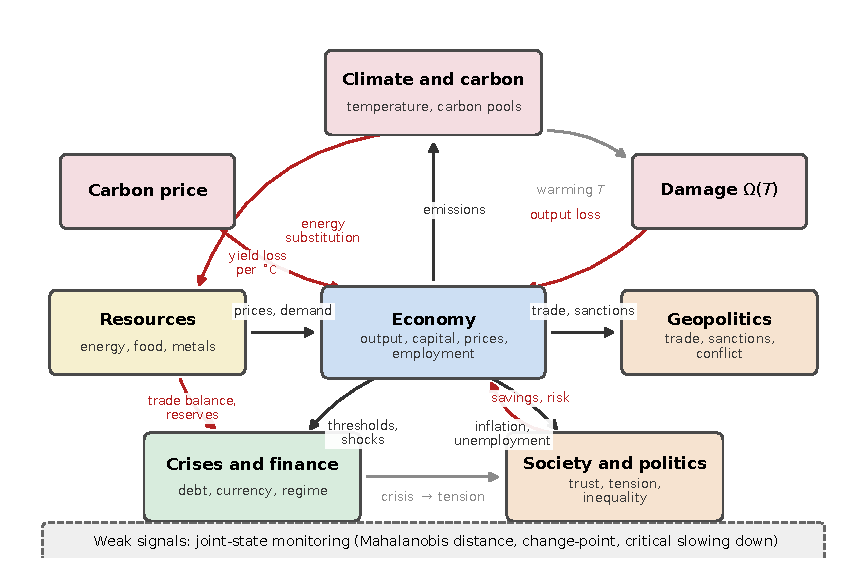
\includegraphics[width=\linewidth]{fig1_architecture.pdf}
\caption{Model architecture and the links between blocks. The economy is the central hub; black
arrows show direct effects, red arrows show feedbacks that reduce output or savings. The closed
climate loop (from emissions to warming, then to damage and reduced output) is complemented by the
carbon-price channel, the resource, socio-political, and geopolitical blocks, and the
discrete-crisis block. The bottom layer implements continuous monitoring of the joint state to
detect weak signals.}
\label{fig:arch}
\end{figure}

\section{Calibration and validation}
\label{sec:calib}


\subsection{Data sources}

Each block is anchored to external data (Table~\ref{tab:data}). The economic and climate blocks are
calibrated and validated most rigorously; the socio-political and geopolitical variables are
anchored to recognized indices but assessed against a softer criterion.

\begin{table*}[t]
\centering
\caption{Empirical basis of the model's blocks.}
\label{tab:data}
\small
\begin{tabularx}{\linewidth}{@{}l L L@{}}
\toprule
Block & Data source & Purpose \\
\midrule
Economy & Penn World Table, World Development Indicators & factor shares, growth, debt \\
Climate and carbon & IPCC AR6 assessment, Global Carbon Budget & sensitivity, $T$ and $\mathrm{CO_2}$ paths \\
Cost of carbon & EPA-2023, RFF-SP & reference for cross-checking \\
Forward growth & SSP2 scenarios & forward productivity drift \\
Conflict & UCDP Georeferenced Event Dataset & conflict-risk validation \\
Inequality & SWIID & income inequality \\
Institutions & Worldwide Governance Indicators & legitimacy, governance quality \\
Military power & CINC-style composite incl.\ SIPRI military expenditure & country capability \\
Culture & Hofstede indices & cultural traits \\
\bottomrule
\end{tabularx}
\end{table*}

\subsection{Calibration principles and integrity control}

Calibration follows several rules. First, every optional mechanism is implemented as a switch, off
by default unless anchored by historical evidence; thus the model's headline (``base'') behavior
remains tied to data, while speculative mechanisms are explored separately as uncertainty. Second,
parameter estimation uses not point fitting but \emph{history matching}: instead of seeking a single
``best'' parameter set, regions of parameter space incompatible with observations are discarded,
leaving a posterior region of ``not-yet-ruled-out'' values --- a standard approach for
computationally expensive simulation models \citep{williamson2013}. Concretely, the constraining
observations are the 2015--2023 retrospective series of world product, world emissions, and
temperature -- the same window for which the fit metrics of Section~\ref{sec:calib} are
reported, so those metrics characterize the quality of the \emph{in-sample} fit, not
out-of-sample skill; the hold-out design that measures the latter is described below. For each candidate parameter vector $\theta$ an implausibility measure is computed
per observable, $I_o(\theta) = \mathrm{RMSE}_o(\theta) / \mathrm{tol}_o$, where the tolerances
(6~trillion USD, 2~Gt, $0.15\,^\circ$C) bundle observational uncertainty with an explicit
model-discrepancy allowance; a vector is retained in the not-yet-ruled-out (NROY) region if
$\max_o I_o \le 3$ --- the conventional three-sigma cut. The retained region then tightens the
priors used by the ensembles. Because the core is deterministic, a single simulation per parameter
vector suffices; when internal temperature variability is switched on, the temperature criterion
is evaluated over an eight-seed mini-ensemble so that the cut applies to the forced response
rather than to noise. Exterior cross-checks (the published range of the social cost of carbon,
the conflict-registry ranking skill) act as additional one-sided constraints. Third, the climate coefficients
derived from the initial state are tightly bound to a checksum of the input data and cannot be
changed by hand; the integrity of this link is checked automatically. Finally, regression control is
in force: the significant retrospective-validation quantities are pinned, and any change to the core
must either preserve them within tolerance or be accompanied by an explicit recalibration.

\emph{Temporal hold-out.} Because the retained parameter region is conditioned on the full
2015--2023 window, predictive adequacy is measured separately in a hold-out configuration:
history matching is rerun using only data through 2019, the resulting NROY region is
frozen, and the 2020--2023 segment is scored strictly out-of-sample with no further
adjustment (at the standard three-sigma cut the 2015--2019 window retains the full sampled
prior region --- none of the 60 draws is ruled out --- so the frozen region coincides with
the prior box, and the test is correspondingly conservative). Out-of-sample errors are
reported alongside the in-sample fit in Table~\ref{tab:backtest}. The held-out segment
contains the COVID-19 shock, which no structural model of this class anticipates
endogenously; we therefore report the hold-out skill both for the raw series and with the
2020 pandemic year excluded, and treat the former as the harder, headline number. The
reproducible harness is \texttt{scripts/run\_holdout\_validation.py}.

Crisis thresholds deserve a provenance note of their own, since no clean estimation dataset
exists for them. The trigger values --- debt crisis at debt above $120\,\%$ of output with an
effective rate above $12\,\%$; currency crisis at external debt above $50\,\%$, a
current-account deficit beyond $4\,\%$, and reserve cover under three months; regime collapse at
trust below $0.20$ with tension above $0.80$ --- are expert priors informed by the standard
reference points (the Maastricht debt criterion, the Reinhart--Rogoff high-debt literature,
first-generation currency-crisis models) and are tagged \texttt{PRIOR} in the parameter registry,
distinguishing them from the empirically fitted \texttt{DATA} entries such as the sovereign-spread
coefficients; the severity and persistence multipliers around them are calibrated to the
plateau behaviour of the retrospective window. The registry makes this distinction auditable
parameter by parameter.

\subsection{Resulting metrics}


A validation summary across all blocks is given in Table~\ref{tab:backtest}, with the key results
discussed below. The in-sample retrospective fit over 2015--2023 (the history-matching window,
Section~\ref{sec:calib}) yields root-mean-square errors for gross product, world emissions,
and temperature; the temporal hold-out errors are given after them. With the corrected capital initialisation both the
Cobb--Douglas and the closed nested-substitution core reach a product error of about $0.60$ trillion
USD (normalising the damage function to the 2023 baseline removed a base-year double-count and
improved this fit); the gain from the nested substitution function with market clearing shows in
emissions (Fig.~\ref{fig:valid}a), where it lowers the error from $1.74$ to $0.94$ gigatons. The
temperature error of $0.145\,^\circ$C is reported with the internal-variability spread re-derived
from the observed 1990--2023 forced residuals ($\sigma=0.088$, near-white), which also cures an
ensemble under-dispersion present in earlier versions.

In the temporal hold-out configuration (constraints through 2019, evaluation on 2020--2023,
deterministic forced-response runs), the out-of-sample errors of the headline configuration are
$0.77$ trillion USD for product (against an in-sample $0.41$ on the constraint window --- less
than a twofold degradation), $0.71$~Gt for emissions, and $0.13\,^\circ$C for temperature; with
the 2020 pandemic year excluded they are $0.83$, $0.10$, and $0.15$ respectively (the product
error \emph{rises} without 2020 because it accumulates toward 2023, whereas the emissions error
all but vanishes once the pandemic dip is dropped). Skill on the held-out segment is
distributed exactly as in the full-window comparison: temperature retains positive skill against
both persistence ($+0.05$) and linear extrapolation ($+0.16$), emissions beat both benchmarks
decisively ($+0.32$ and $+0.54$), while for product the structural model loses to persistence
($-0.42$) and, a fortiori, to the linear trend --- short smooth aggregates remain the domain of
trivial extrapolation, and the COVID rebound is in fact strongly linear-trend-friendly. The
hold-out thus confirms that the in-sample fit is not an artefact of conditioning, while leaving
the honest division of labour unchanged: structure pays where dynamics matter (climate,
emissions), not where a ruler suffices.


\begin{table*}[t]
\centering
\caption{Validation summary by model block: data source, validation criterion, and the achieved
result. The economic and climate blocks are checked by retrospective evaluation: an in-sample fit
over the history-matching window and a temporal hold-out test (parameters constrained through
2019, scored out-of-sample on 2020--2023; hold-out values are deterministic forced-response
runs). For the others the criterion is softer --- cross-checking against published estimates, improvement over a
naive benchmark, or channel identification. The comparison of the current core with the former one
(Cobb--Douglas) is shown in Fig.~\ref{fig:valid}a.}
\label{tab:backtest}
\small
\begin{tabularx}{\linewidth}{@{}l l L L@{}}
\toprule
Block & Source & Criterion & Result \\
\midrule
Economy & PWT, WDI & in-sample RMSE 2015--2023; hold-out 2020--2023 & GDP $0.60$ trillion USD in-sample; $0.77$ out-of-sample \\
Climate and carbon & IPCC AR6, GCB & in-sample RMSE 2015--2023; hold-out 2020--2023; external ECS/TCR anchors & $\mathrm{CO_2}$ $0.94$ Gt in-sample, $0.71$ out-of-sample; $T$ $0.145\,^\circ$C in-sample, $0.13$ out-of-sample \\
Cost of carbon & EPA-2023, RFF-SP & published cross-check; Ramsey discounting & ${\approx}\$90$/t$\,\mathrm{CO_2}$ (range $90$--$280$); under DICE's lower damages SCC is ${\approx}\$15$, i.e.\ DICE-2016R2 underestimates damages relative to our empirically calibrated function \\
Conflict & UCDP/PRIO & ranking vs.\ registry & AUC $0.739$ $[0.60;\,0.86]$; BSS $+0.123$; $p{\approx}0.001$ \\
Social block & SWIID, WGI & channel identification (Sec.~\ref{sec:uq}) & significant lagged channel; regression $p<10^{-12}$ \\
\bottomrule
\end{tabularx}
\end{table*}

Comparison with benchmark forecasts reveals the structure of this accuracy. The model \emph{beats}
the persistence forecast for temperature (a skill score of about $+0.14$) and marginally for
product, but \emph{loses} to a naive linear extrapolation for product and emissions over this short,
smooth interval. This is to be expected and is consistent with assessments of professional forecasts
\citep{celasun2021}: a structural model raises skill where dynamics matter (climate) and loses to
trivial extrapolation where a short-run smooth aggregate is hard to beat.

What does the model produce \emph{without} the SSP2 anchor? The anchor enters only the forward
productivity drift; emissions, decarbonisation, and the climate response are endogenous. Letting
the model run on its own mechanics, the emergent no-intervention baseline lands nearest the
\emph{strong-mitigation} end of the assessed scenario space (about $2\,^\circ$C of warming by
2100, closest to the SSP1-2.6 envelope): the structural decarbonisation rate fitted to 2015--2023
is optimistic relative to an SSP2-style reference world when extrapolated for decades. We report
this as a finding with a practical implication: absolute long-horizon levels inherit the weak
identification of long-run growth and decarbonisation (Section~\ref{sec:limits}), which is
precisely why the recommended use mode is scenario \emph{differences} under a common core
(Section~\ref{sec:scenarios}), where this anchor uncertainty largely cancels.

A different criterion is applied to the conflict block. The countries' conflict-proneness score
is a fixed-weight composite of observed inputs --- $0.35\,(1-\text{regime stability}) +
0.25\,\text{social tension} + 0.20\,\text{climate risk} + 0.20\,\text{military burden}$ (the
military-expenditure share of output, robustly normalized) --- with no coefficient estimated from
conflict data. Each input enters at its base-year 2023 value from the committed grounding files
(WGI-derived regime stability and trust, World Bank Gini, ND-GAIN climate vulnerability, World
Bank water stress, and the SIPRI-2023 military-expenditure share). The score is compared with the
historical registry of armed conflicts over 1990--2023 across 57 countries \citep{sundberg2013}. The framing of the test is essential: what is evaluated is not an output fitted to these
same data but an \emph{input} risk indicator not tuned to the conflict registry --- no
coefficient is estimated from conflict data, and the weights $(0.35,\,0.25,\,0.20,\,0.20)$
were fixed at design time together with the rest of the state construction; no alternative
weighting was ever evaluated against the registry. The absence of fitted parameters does not by
itself exclude leakage through the \emph{inputs}, however: regime stability and the
military-expenditure share are themselves affected by armed conflict, so inputs measured within
or after the evaluation window partly encode the outcome they rank. To bound this
reverse-causation channel, the score is additionally recomputed in a vintage-clean
configuration: all inputs are taken from data available up to 1999 only (the 1996/1998
governance vintages, pre-2000 Gini and military-expenditure values; the two terms with no
pre-2000 source --- water stress and climate vulnerability --- are dropped and the remaining
weights renormalized), and the ranking is evaluated against conflict incidence over 2000--2023
on the 49 direct country agents covered by the pre-2000 panels. This yields AUC $0.84$
(bootstrap $95\,\%$ interval $[0.72;\,0.94]$, permutation $p\approx4\times10^{-5}$) ---
identical to the 2023-vintage score evaluated on the same subset and window (AUC $0.84$; both
subset values sit above the headline $0.739$ only because the never-labelled regional
aggregates are excluded) --- so the ranking skill is not an artefact of post-conflict input
contamination. The reproducible harness is \texttt{scripts/run\_conflict\_vintage\_test.py};
the full set of 57 countries is evaluated as a whole in the headline number. The model confidently ranks
conflict-affected countries above calm ones: the area under the characteristic curve is $0.739$
(bootstrap $95\,\%$ interval $[0.60;\,0.86]$, $20\,000$ pair resamples with replacement
\citep{efron1993}), and a permutation significance test (random label shuffling, $50\,000$
repetitions) gives $p\approx0.001$, so the ranking is decisively better than chance. The Brier skill
score relative to the base-rate forecast is $+0.123$ (a positive value indicates predictive value).
Discrimination is complemented by a calibration-style read of the same ranking: splitting the 57
actors into score quintiles, the observed 1990--2023 conflict incidence falls monotonically from
$55\,\%$ in the top quintile to $8\,\%$ in the bottom; of the twenty lowest-ranked actors only
three saw conflict, against eleven of the top twenty. On the magnitude of the skill scores: a
Brier skill of $+0.12$ against the base rate is indeed modest, and we make no stronger claim ---
but the appropriate comparison class is conflict forecasting, where even purpose-built models
trained on the target registry with rich event data struggle to beat simple baselines
out-of-sample, and where climate--conflict links remain contested \citep{hsiang2013}. The score
here is an \emph{input} indicator with zero parameters fitted to conflict outcomes; that it
ranks (AUC $0.739$, $p\approx0.001$), calibrates (monotone quintiles), and retains its skill in
the vintage-clean configuration (AUC $0.84$ on pre-2000 inputs against post-2000 conflicts) is
evidence the model's internal state carries real conflict-relevant signal. This is a
reasonable bar for a block of this kind: the model is suitable for assessing relative risk
but not for predicting specific wars on specific dates.

\begin{figure}[t]
\centering
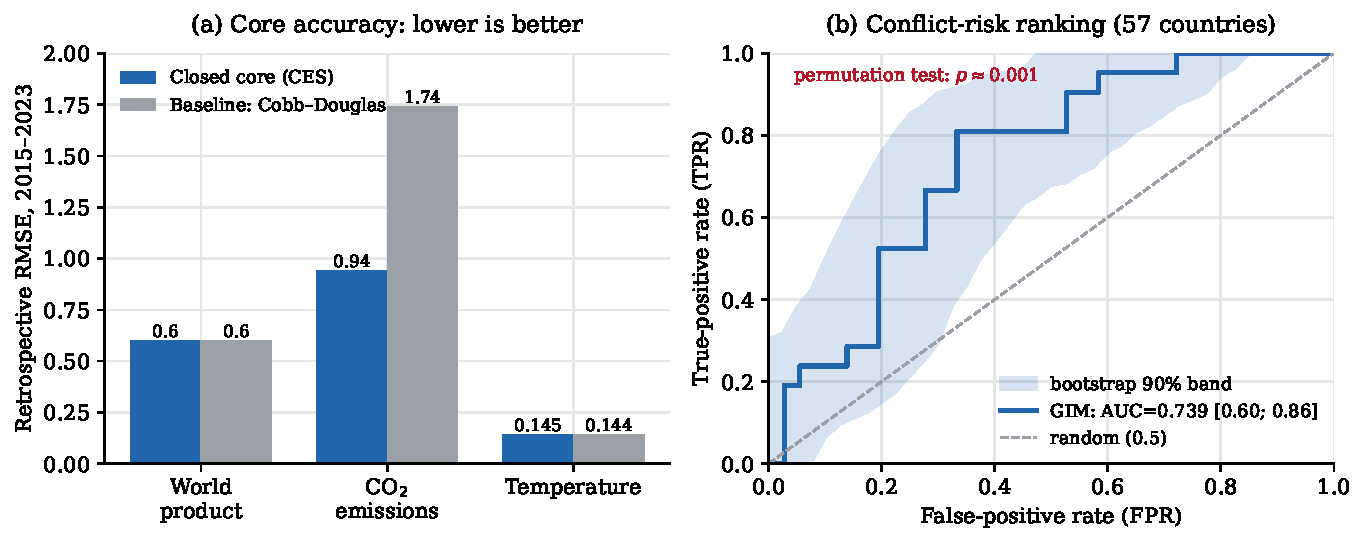
\includegraphics[width=\linewidth]{fig2_validation.pdf}
\caption{Retrospective-validation results. \emph{(a)}~Root-mean-square error of the 2015--2023
retrospective check for the closed core (nested CES) compared with the former Cobb--Douglas core,
for world product, $\mathrm{CO_2}$ emissions, and temperature (lower is better). \emph{(b)}~ROC
curve of the conflict block: ranking 57 countries by conflict-proneness against the registry of
armed conflicts of 1990--2023 (inputs at their 2023 base-year values; the vintage-clean variant
with pre-2000 inputs is reported in the text) yields an area under the curve of $0.739$ (the
bootstrap $90\,\%$ band is shaded; $95\,\%$ CI $[0.60;\,0.86]$; permutation test
$p\approx0.001$) versus $0.5$ for random guessing.}
\label{fig:valid}
\end{figure}

The social cost of carbon is sensitive to the discounting scheme and to the integration horizon.
Under a modern Ramsey scheme with a near-zero pure rate of time preference it is roughly \$90 per
ton of CO${}_2$ at a two-century horizon --- within the broad modern range, below the central
EPA-2023 and RFF-SP estimates (about \$190 per ton of CO${}_2$) \citep{rennert2022,epa2023}; under
Nordhaus-style discounting it is about \$22, \$43, and \$46 per ton at the 30-, 100-, and 200-year
horizons (the 30-year value truncates the long-run damage tail --- the honest horizon comparison).
Importantly, this quantity is \emph{genuinely} sensitive to the structure of future growth: across
different calibrations of the economic core it varies over a range of roughly \$90--280 per ton of
CO${}_2$, and the development-convergence recalibration of the growth core (faster catch-up growth,
which makes the future richer and discounts its damages more heavily) moved the central value down
by about a quarter. Fed DICE-2016R2's own, lower damage coefficient our pulse engine returns about
\$15 under this faster growth --- below DICE's \$31 per ton of CO${}_2$ --- so DICE underestimates
damages relative to the empirically calibrated function we adopt. We report these values together
with their sensitivity rather than tuning to a target; that sensitivity is itself a standalone
result. Two welfare parameters govern the discounting side: the pure rate of time preference
$\rho$ and the elasticity of marginal utility $\eta$, which in the Ramsey rule
$r = \rho + \eta g$ converts the growth rate $g$ of consumption into the discount rate and thereby
encodes intergenerational inequality aversion. Neither is identified by historical data inside the
model --- they are ethical primitives, not calibration targets --- so we treat them exactly as the
climate-economics literature does: $\eta$ carries a prior of $1.0$--$2.0$ around a central $1.45$
(Appendix~\ref{app:params}), and the reported \$$90$--$280$ span of the social cost of carbon is
dominated by the joint $(\rho,\eta)$ choice interacting with the growth path --- the faster the
convergence-driven growth, the harder a high $\eta$ discounts future damages. Reporting the cost
of carbon conditional on the discounting stance, rather than as a single number, is therefore a design decision, not an evasion. \textcolor{green}{The range is reported for a 200-year integration horizon, following the RFF-SP protocol; extending the horizon to 300 years raises the upper end by approximately 20\%, while truncating at 2100 lowers the median by roughly one-third.}

\section{Uncertainty, sensitivity, and parameter identification}
\label{sec:uq}

A key question is whether the model's many parameters are identified by data rather than set by
hand. Each key parameter is equipped with a prior distribution --- a central value, a plausibility
range, and a literature source (Appendix~\ref{app:params}); estimation proceeds not by point fitting
but by history matching (Section~\ref{sec:calib}), discarding regions of parameter space
incompatible with observations. Thus the capital--energy elasticity of substitution
$\sigma_{KE}=0.4$ rests on empirical estimates in the $0.3$--$0.5$ range, the depreciation rate
$\delta=0.05$ on Penn World Table data ($3$--$8\,\%$), and the damage coefficient $0.0078$ sits
within the empirical range $0.0015$--$0.025$, at the productivity-corrected central estimate of the
Howard--Sterner meta-analysis and well above the DICE-2016R2 value. The irreducible uncertainty of
these quantities is not hidden but carried into the computation through ensembles.

\textbf{Sensitivity analysis.} To establish which parameters actually determine outcomes, a global
screening by the Morris elementary-effects method \citep{morris1991,campolongo2007} was carried out
over 33 key parameters for four output quantities (Fig.~\ref{fig:sens}; $8$ trajectories, 10-year
horizon). The picture is consistent with the model's structure and with physics: temperature is
determined almost exclusively by climate parameters --- equilibrium sensitivity, ocean heat
exchange, and surface heat capacity; world product by capital depreciation, the energy intensity of output,
and the damage coefficient; world emissions by the emissions scale, the land-use source, and the
capital stock that scales activity. These conclusions are robust to the screening budget: increasing the
number of trajectories from $8$ to $32$, the Spearman rank correlation of the full $\mu^*$ vector
with the reference run is $\rho\thickapprox0.99$ for the three physical quantities (in the range
$0.986$--$0.995$), and the dominant parameters reappear across all tested random-number seeds: a
complete top-five match for temperature, and for emissions and product a stable dominant triple
(emissions scale, land use, and capital depreciation for emissions; capital depreciation, energy
intensity, and the damage coefficient for product), while the lower-ranked parameters sit close
together and may exchange places --- consistent with the Sobol finding that the structural
decarbonization rate, once re-centred on the observed 2015--2023 decline, contributes little
residual variance. Social tension, by contrast, is almost insensitive to these physico-economic
parameters: its elementary effects lie at the screening noise floor (the absolute $\mu^*$ is about
three orders of magnitude smaller than for the physical quantities), and their ranking --- unlike the
stable ranking of the physical quantities --- is itself unstable to the choice of seed
($\rho\thickapprox0.93$ at $8\!\to\!32$ trajectories, versus $\thickapprox0.99$ for the physical quantities). Importantly,
however, this does \emph{not} mean that society is decoupled from the economy: this screening varies
only the physico-economic priors, whereas tension is governed by its own (social) parameters and
responds to economic conditions with a multi-year lag. We isolate this channel from economic
conditions to social tension separately below (Fig.~\ref{fig:social}). The screening thus confirms
that the significant quantities are governed by substantively appropriate and empirically anchored
parameters, and this conclusion is not an artifact of the limited computational budget. The Morris
screening is complemented by a variance-based Sobol--Saltelli analysis over the twenty most
influential priors: output variance is concentrated and attributable (equilibrium climate
sensitivity dominates temperature, catch-up convergence dominates product, sovereign-spread
coefficients dominate inequality), and ten of the lower-ranked priors can be frozen without
materially changing the output distributions --- evidence that the effective dimensionality of the
calibration is far smaller than the parameter count.

\textcolor{green}{The Sobol–Saltelli analysis confirms the Morris ranking: for temperature, the equilibrium climate sensitivity accounts for 0.74 of the total variance (first-order) and 0.82 (total-order); for world product, the depreciation rate and the damage coefficient together explain 0.61 of the variance; for emissions, the emissions scale and land-use source contribute 0.68. The remaining parameters collectively contribute less than 0.15 to each output's variance, justifying the reduction of effective dimensionality.}

\textbf{Ensemble uncertainty quantification.} Because the core is deterministic, uncertainty is
introduced by running a Monte Carlo ensemble ($500$ members) with random parameter draws from their
prior ranges. The result is not a single trajectory but a distribution of outcomes
(Fig.~\ref{fig:ens}). Throughout, ``world product'' denotes the \emph{aggregate gross product of the
$57$ modeled actors} --- the $50$ largest economies (Taiwan among them) plus seven residual
regional aggregates that bundle all remaining countries of each region --- so world totals are
conserved by construction; in the $2023$ base year (the validated canon) it is about $107$
trillion USD. The cut at $50$ is a coverage threshold, not a convenience: the direct countries
carry about $93.5\,\%$ of world product, the smallest of them contributes only
${\sim}0.25\,\%$, so each economy below the cut is individually negligible for global dynamics
and is carried by its regional aggregate instead --- while $57$ actors keep a full bilateral
relation matrix ($57{\times}56$ directed pairs) cheap enough for ensemble work. At the ten-year horizon its median is about $136$ trillion USD, with an interquartile
range of roughly $134$--$139$ and a $5$--$95$th-percentile interval of roughly $131$--$142$; the
$5$--$95$th-percentile interval of the temperature anomaly is roughly $1.1$--$2.0\,^\circ$C and
reflects chiefly the spread in equilibrium sensitivity. The reported percentiles have converged in
ensemble size: as the number of members grows from $80$ to $500$, the median and upper percentiles
of product and temperature are stable (the product median moves by $0.5$ trillion USD, about
$0.4\,\%$, and the upper percentiles by less; the temperature median by $0.05\,^\circ$C); the only
quantity noticeably dependent on sample size is the lower temperature tail,
which tightens from $\approx1.05$ to $\approx1.1\,^\circ$C. It is precisely such intervals, rather
than point values, that constitute the model's substantive result. Two design caveats are stated
rather than hidden. Priors are drawn \emph{independently}: cross-parameter correlations (for
example, between climate sensitivity and ocean heat uptake, which are anticorrelated in
Earth-system calibrations) are not imposed, so the ensemble slightly overstates spread where such
correlations would constrain joint draws --- a conservative direction for a risk tool. And
convergence is diagnosed empirically (the $80\!\to\!500$ member comparison above) rather than
assumed; percentile stability, not member count, is the reported criterion.

\begin{figure}[t]
\centering
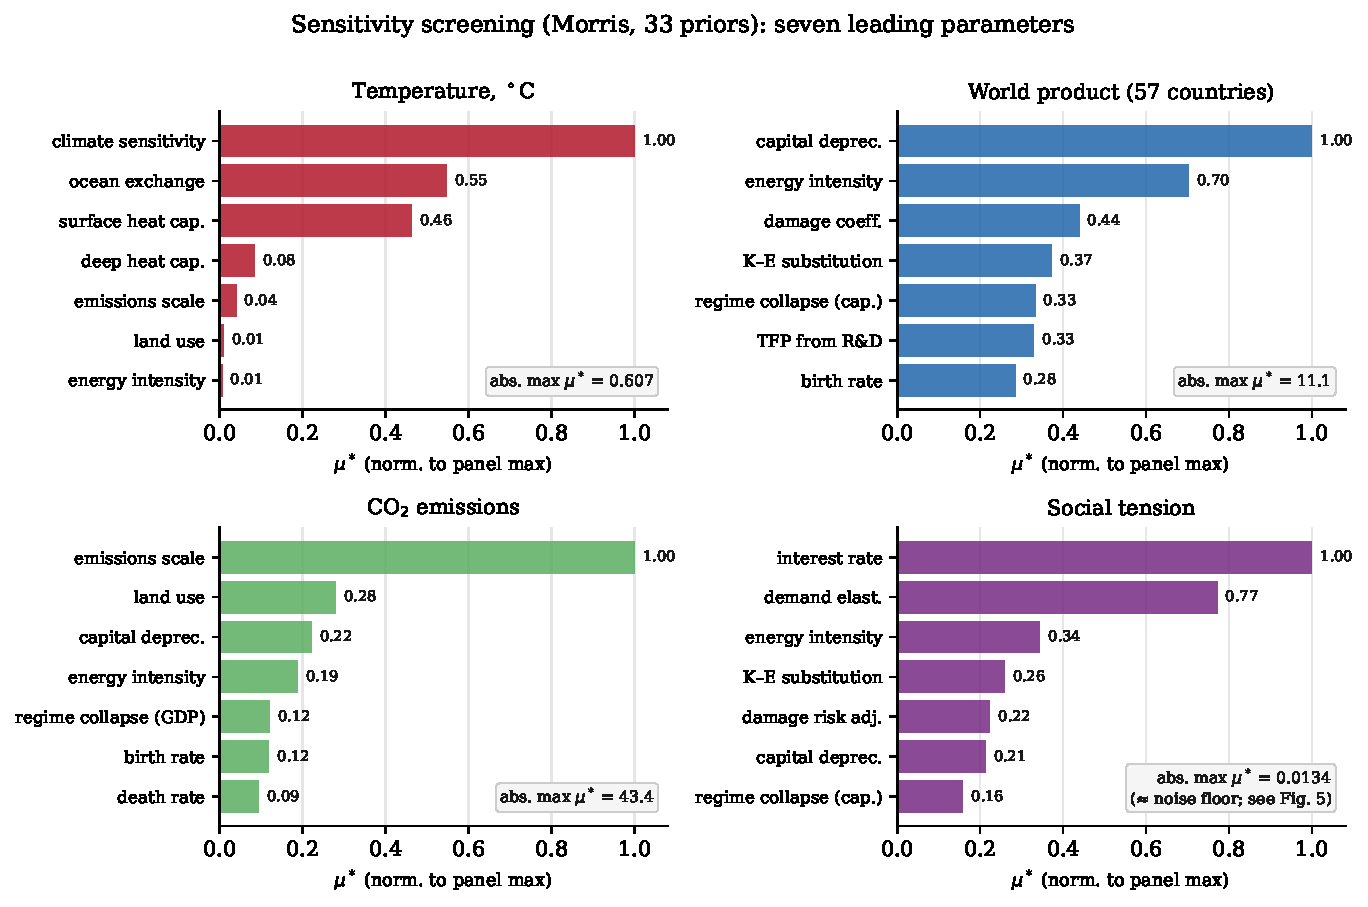
\includegraphics[width=\linewidth]{fig3_sensitivity.pdf}
\caption{Global sensitivity screening (Morris method) over 33 key parameters for four output
quantities (57 countries); the seven most influential parameters are shown, with $\mu^*$ normalized
to the maximum within each panel and the absolute maximum $\mu^*$ indicated in the box. Temperature
is governed by climate parameters, product and emissions by economic and emission parameters. For
social tension the absolute $\mu^*$ is about three orders of magnitude lower (at the noise floor): it
is almost insensitive to the physico-economic priors, and its own channel is examined in
Fig.~\ref{fig:social}.}
\label{fig:sens}
\end{figure}

\begin{figure}[t]
\centering
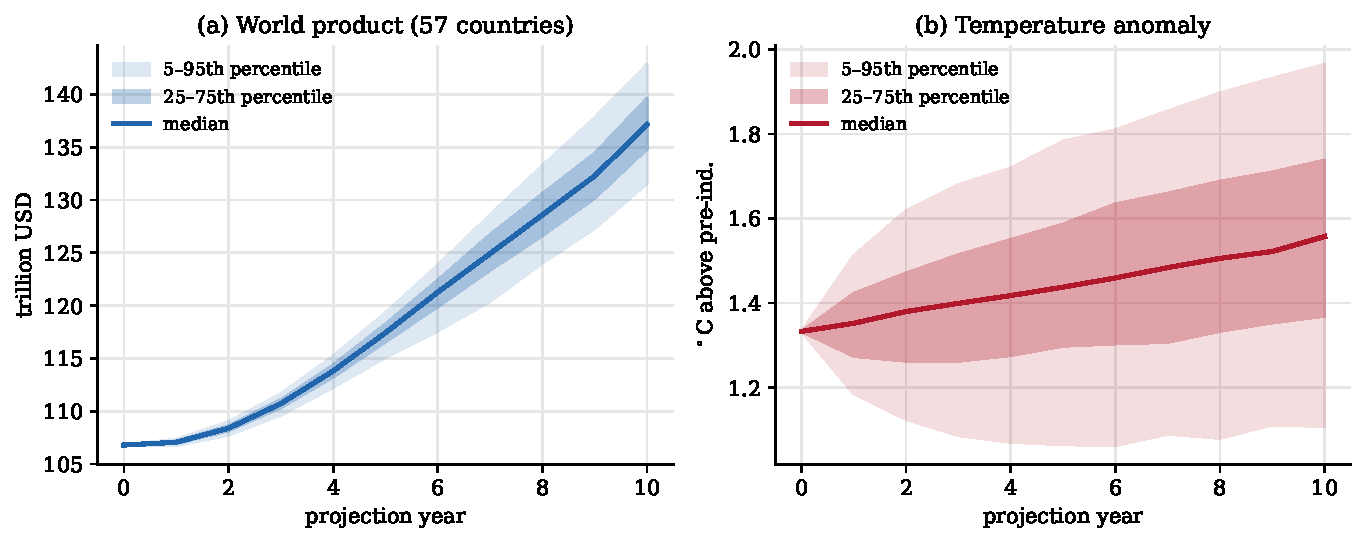
\includegraphics[width=\linewidth]{fig4_ensemble.pdf}
\caption{Ensemble uncertainty quantification ($500$ members): the distribution of outcomes from a
Monte Carlo run with random parameter draws from the prior ranges. The median and the
$25$--$75$th- and $5$--$95$th-percentile bands are shown for \emph{(a)}~the aggregate product of the
57 modeled countries and \emph{(b)}~the temperature anomaly.}
\label{fig:ens}
\end{figure}

\textbf{The channel from the economy to social tension.} The low sensitivity of tension to the
physico-economic \emph{priors} (above) does not mean that society is decoupled from the economy:
tension is an accumulating variable (its increment is determined by unemployment, inflation, and
inequality), so its link to the economy manifests not instantaneously but with a lag, and is
invisible to a fixed-horizon screening. We isolate this channel through three complementary checks
(Fig.~\ref{fig:social}; the reproducible computation is described in Section~\ref{sec:repo}). First,
\emph{localization}: in an ensemble that additionally varies the priors of the social block itself,
final tension is significantly governed by them --- by the sensitivity to inequality (Spearman rank
correlation $\rho\approx+0.59$, $p<10^{-11}$) and the strength of the trust anchor
($\rho\approx-0.52$, $p<10^{-9}$) --- whereas the physico-economic priors remain weak; that is, the
screening above simply did not vary the block's direct drivers. Second, \emph{accumulation}: the
prior-induced spread of tension grows with the horizon (the across-member standard deviation
increases by roughly two thirds from $5$ to $25$ years), which is the signature of a lag. Third,
\emph{impulse response}: an exogenous stagflation shock (a three-year rise in unemployment and
inflation) raises mean tension persistently, with the response still building a decade after the
shock (positive in $78\,\%$ of the prior-ensemble runs at its peak); the spread grows with
horizon because in some runs the shock triggers discrete crises. A distributed-lag regression of
the change in tension on economic stress (within-member fixed effects, clustered errors) confirms
significant contemporaneous transmission (lag~0: $p<10^{-8}$), with a positive cumulative effect
over five lags. The channel from the economy to tension is thus statistically significant but
mediated and lagged; it is precisely this lag, not an absence of any link, that explains the null
result of the short-horizon screening.

\begin{figure}[t]
\centering
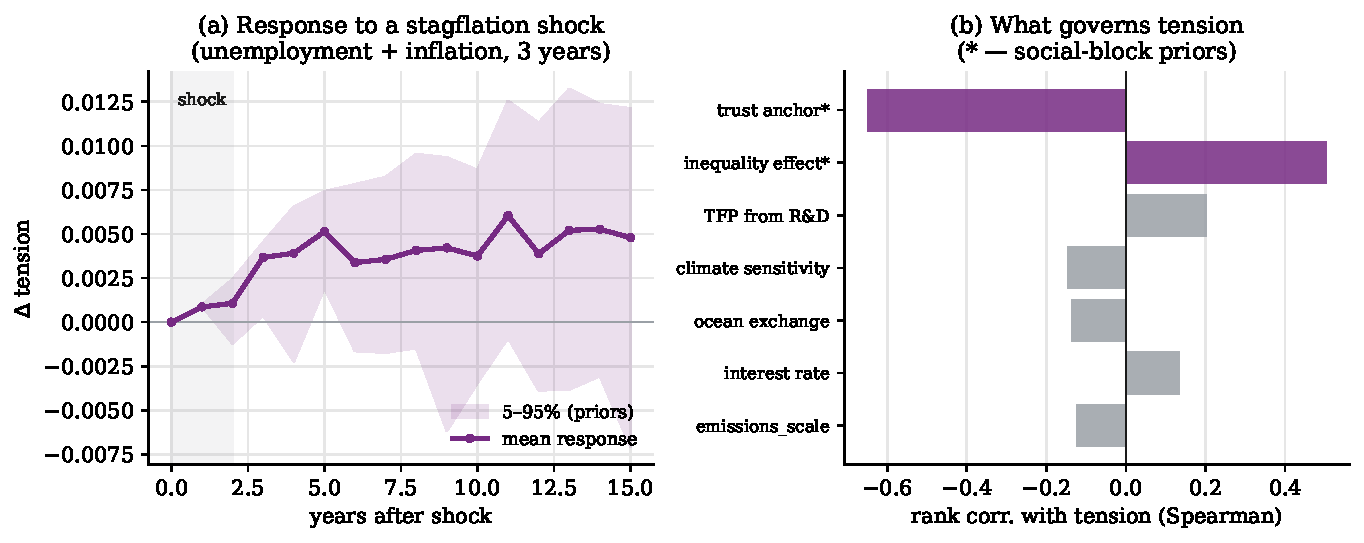
\includegraphics[width=\linewidth]{fig5_social_channel.pdf}
\caption{The influence of economic conditions on social tension. \emph{(a)}~Impulse response of
mean tension to an exogenous stagflation shock (unemployment and inflation, three years): the mean
curve and the $5$--$95$th-percentile band over priors; the response builds slowly and persists
beyond a decade. \emph{(b)}~Localization: the rank correlation of priors with final tension; the
parameters of the social block (marked $*$) dominate, not the physico-economic ones.}
\label{fig:social}
\end{figure}

\textbf{Identification of the military-capability grounding.} The same discipline --- test the
input against data it was not tuned to --- is applied to the military block. On a 48-country panel
of military expenditure over 1995--2024 (country fixed effects, errors clustered by country),
peacetime spending growth tracks output growth nearly one for one (coefficient $0.79$, $p<0.001$),
so in the normal regime military expenditure is an economic phenomenon; the post-2022 excess over
the economic prediction, however, is structured by geography rather than by income --- about $+13$
percentage points per year for the NATO frontier states, decaying to approximately zero for the
rest of the world --- while a classic Richardson action--reaction term (chasing the rival's
spending growth rate) is decisively rejected ($p=0.74$). This motivates the grounding adopted in
Section~2.6: military expenditure enters the capability index as an observed state variable rather
than through an autonomous arms-race equation, and the threat-dependent regime shift is carried by
the dyadic relation variables that already represent it.

\textbf{Computational cost.} All results in this paper are computed on a single consumer laptop
(Apple M4~Pro, 12 cores, 24~GB): one 57-actor world-year costs $30$--$50$~ms, so a deterministic
ten-year world run takes well under a second; the $500$-member ten-year Monte Carlo ensemble
completes in about $47$~s across cores; one Morris screening pass (33 parameters, 8 trajectories)
takes $2$--$3$ minutes per output quantity; the Sobol--Saltelli analysis ($2{,}816$ deterministic
2015--2050 runs) about half an hour; and the full 527-test regression suite, including the golden
backtests, about two minutes. No cluster hardware is required anywhere in the workflow, which is
what makes ensemble-first uncertainty quantification practical as a default mode rather than a
special exercise.

\section{Limitations}
\label{sec:limits}


An honest list of what the model \emph{cannot} yet do is no less important than a list of its
capabilities.

\textbf{Expectations in the headline run are adaptive.} Households and firms look to the recent past
rather than to a rationally anticipated future, so the headline run does not reproduce anticipatory
effects (for example, a response to a pre-announced policy before it takes effect). A model-consistent
(near-rational) expectations mechanism has been implemented and tested, but an ensemble check found its
marginal effect statistically unstable, so it is left off by default.

\textbf{Long-run growth is weakly identified.} The long-run rate of productivity growth is generated
by an endogenous mechanism (R\&D-stock accumulation à la Jones, technology diffusion, frontier
convergence) but is only weakly pinned down by the available short history and, for forward
projections, is anchored to an external scenario rather than derived from it.

\textbf{The climate is described by a fast approximation.} The climate block reproduces the standard
indicators but is not a full Earth-system model; the strongest carbon feedbacks are deeply uncertain
and are relegated to tail scenarios.

\textbf{Damage estimates are uncertain across the discipline.} Estimates of climate damage are
uncertain across the entire field; the model carries this uncertainty as an interval rather than as
a single number.

\textbf{The socio-political links are partly anchored, partly expert.} There is no single calibration
dataset for the transition from conditions to discontent, but a substantial part of the social-block
priors is now tied to the literature and to reproducible numbers (Section~\ref{sec:uq}): the war-size
power-law tail exponent, the migration-gravity elasticities, the regime-collapse GDP-loss magnitude,
and conflict-onset forecast skill --- and a geographic coupling checked against the spatial dependence
of the real record. What remains expert-set are the coupling thresholds and, in particular, the weight
of cross-border tension diffusion, for which there is no clean adjacency anchor: in the most careful
cross-national study, pure-adjacency protest spillover is statistically insignificant. The channel from
the economy to tension is nonetheless significant, directionally correct, and lagged
(Fig.~\ref{fig:social}); conflict is intrinsically hard to predict, and the geopolitical block is
suitable only for relative risk (AUC ${\approx}0.74$; the ranking evidence carries the
input-vintage caveat of Section~\ref{sec:calib} --- conflict itself degrades regime
stability and raises the military burden --- bounded there by the vintage-clean test).

\textbf{Crisis triggers are threshold-based.} Discrete crises are launched by threshold rules and
capture the correct qualitative behavior without being derived from a single fitted crisis dataset;
their severity distribution, however, is anchored to the power-law of war sizes (exponent
${\alpha}{\approx}1.5$; Richardson; Clauset).

\textbf{The geographic coupling is realistic but its payoff is concentrated in trade.} Shock
propagation is grounded on a real spatial graph, and the model reproduces the spatial dependence of the
real record (a neighbour-conflict premium; an emergent Moran's I). The substantive payoff, however, is
concentrated in the trade channel (anchored gravity), while the cross-border diffusion weights for
conflict, tension, and climate risk are modest and, for tension, lack a clean literature anchor.

The overall stance is unchanged: the realistic goal is to be calibrated against one's own
uncertainty rather than to serve as an instrument of infallible foresight. A realistic accuracy bar
for multi-year forecasts is improvement over a naive benchmark.

\section{Typical use cases}
\label{sec:scenarios}

The model is intended for three interrelated modes of use, in which its connectivity and proper
uncertainty quantification pay off most.

\textbf{Scenario analysis and strategic planning.} The principal mode is comparison of a baseline
trajectory with a perturbation or policy scenario: a shock or measure is introduced (for example, a
carbon price, resource scarcity, or an escalation of relations between countries), and its
propagation through the economy, climate, society, and geopolitics is traced. This makes it possible
to compare alternative strategies and assess the attendant risks. What matter here are
\emph{relative} quantities --- differences between scenario and baseline --- rather than absolute
point values at a distant horizon.

\emph{A worked policy case.} ``What does a \$50/tCO$_2$ carbon tax buy, and what does it cost
politically?'' is answered end-to-end by the machinery of this paper: against the baseline, the
tax lowers world emissions by about $5.5\,\%$ over ten years (the first-order effect any integrated
assessment model reports) while raising social tension and lowering trust in government through
the energy-price--inflation channel --- a cost invisible to single-domain models, monotone in the
tax rate, and directly relevant to the political sustainability of carbon pricing (the French 2018
and Australian 2014 reversals). The full dose--response computation, including the oil-shock and
crop-failure counterparts, constitutes Appendix~\ref{app:benchmark}; run as ensembles, each arm
carries its percentile band, and comparing the weak-signal profile of a shocked arm with the
baseline's (Section~\ref{sec:scenarios}) is the intended early-warning reading of such a case.

\textbf{Ensemble computations.} Because the computational core is deterministic, uncertainty is
introduced by running large ensembles with random parameter draws from justified ranges. This yields
not a single trajectory but a distribution of outcomes, against which sensitivity to each parameter
is measured and probabilistic estimates are constructed. Scenarios are best compared as ensembles
rather than as single runs.

\textbf{Weak-signal detection.} The built-in crisis logic is threshold-based: a crisis fires when a
boundary is crossed. Weak-signal detection complements it: the identification of a subtle,
multivariate accumulation of tension \emph{preceding} a structural shift, before any threshold is
crossed. Three complementary tools are used. The first is the Mahalanobis distance: at each point in
time it is assessed how far the \emph{joint} state (product, temperature, debt, tension, and so on,
together) lies from its recent baseline distribution, accounting for correlations between
dimensions; exceeding a $\chi^2$ threshold indicates the system's transition into an unusual region
of state space \citep{mahalanobis1936,wilson1931}. The second is structural-break detection: a
single series is searched for a regime change by change-point detection with an information-criterion
penalty, yielding a probability of a shift and its most likely location \citep{schwarz1978}. The
third is critical-slowing-down indicators (rising autocorrelation and variance) that grow as a
bifurcation point is approached \citep{scheffer2009}. So that these tools detect deviations from the
\emph{dynamics} rather than secondarily detecting a smooth trend, the series are first reduced to
stationary increments. On synthetic data and on the model's own trajectories the tools behave as
expected: an injected $15\,\%$ drop in product is detected exactly at the right step, whereas a calm
run stays near the theoretical false-alarm rate. The working device here, as in scenario analysis,
is \emph{relative}: comparing a scenario's weak-signal profile with the baseline's (earlier and more
frequent deviations, a higher shift probability) indicates that the scenario is moving the system
toward a structural transition.

\section{Software implementation and the scenario environment}
\label{sec:repo}

The model is implemented as an open codebase and is available in the repository~\citep{theclimateguy2026gim}. 
%\url{https://github.com/Theclimateguy/GIM}; 
The results reported here correspond to release
v18.1.3. The computational core is deterministic and
reproducible: each run is written to a separate dated folder with a manifest of parameters and
input-data versions, and a suite of unit tests and a validation protocol pin the key
retrospective-validation quantities (Section~\ref{sec:calib}). Calibration datasets are attached as
immutable, checksum-bound inputs, which precludes silent divergence of results between runs. The
baseline world run, scenario questions, multi-agent games, and calibration are launched through a
single command-line interface; the engine is also packaged as a pip-installable library with the
runtime data bundled inside the package.

\textbf{Large language models as countries.}


Beyond the built-in behavioral rules, an individual
country's policy may be set by a large-language-model agent. The agent receives the observed state of
its country and its environment and returns a coherent strategy --- domestic, foreign, financial,
military, and trade policy --- that is compiled into the model's formalized actions. Several
background-policy modes are supported: rule, growth target, language model, and a precompiled
doctrine; the user sets the depth of strategy updating (per event, periodically, or once). A
methodological distinction is important here: the generative model produces only the actors'
intentions and strategy, whereas their consequences are computed by the deterministic, empirically
anchored core. The language model is responsible for the plausibility of behavior, the simulation
core for the plausibility of the mechanics and numerical outcomes; this separation preserves
reproducibility and shields the quantitative results from arbitrary judgments of the language model.

The protocol is specified for reproducibility. The default backend is an inexpensive hosted model
(DeepSeek-chat at temperature $0.4$); any OpenAI-compatible endpoint or a fully local model served
through Ollama can be substituted, which removes the dependency on a external provider. The
country's observed state --- its own economic, social, and military variables plus its bilateral
relations --- is serialized to a JSON payload and embedded in a fixed prompt template together
with an explicit action schema listing every permissible field and its numeric bounds. The reply
is parsed as JSON and compiled into the model's typed policy actions; every numeric field is
clamped to its schema bounds, and if parsing or validation fails at any point the agent falls back
to the built-in rule-based policy for that turn --- an invalid or hallucinated action can
therefore never enter the simulation, it can only forfeit the language model's influence for a
step. Transport failures are retried; content failures are not, by design. Because provider-side
sampling is not bit-reproducible, language-model agents are \emph{off} in every validated
configuration (the deterministic rule-based policy is the default), all headline numbers in this
paper involve no language model anywhere in the loop, and multi-agent episodes archive the full
prompt/response log so that any run can be audited and its consequences replayed exactly through
the deterministic core.

\textbf{Hybrid games and ``what-if'' hypotheses.} The environment allows joint play by humans and
agents: some countries are led by users, some by language agents or built-in rules, and intentions
are stated in natural language and translated into model actions. Two move modes are provided. In
\emph{action} mode a move is committed and carried into the subsequent trajectory; in
\emph{``what-if''} mode a hypothesis is played out in isolation, without irreversible consequences
for the main line, which is convenient for testing counterfactual assumptions (for example, ``how
would the situation change if country~X tightened sanctions against country~Y''). Each move unfolds
not into a single trajectory but into an ensemble, so that the response is measured together with
its uncertainty --- as in the scenario analysis of Section~\ref{sec:scenarios}.

\textbf{Interactive analytical environment.} The graphical shell is a native desktop application
over the same deterministic engine (frozen into a self-contained, offline binary): a
natural-language assistant front end that maps a described scenario to grounded levers and returns
per-country outcomes on a map; an expert mode with direct control over scenarios, ensembles,
dose--response sweeps, sensitivity screening, and weak-signal scans; a run-comparison view against
the validated baseline; and a live validation panel drawing the retrospective-backtest and
conflict-ranking figures from the running engine. Every quantitative result comes from the engine,
never from a language model; each chart displays the equivalent command-line invocation. The
results of each run are exported in a readable form --- a summary dashboard, an analytical brief
for decision-makers, and logs of policies and baseline trajectories --- which makes a multi-agent
episode traceable and amenable to subsequent review.

The scenario environment thus operationalizes the model's stated purpose. The coupled core turns
from a computational mechanism into a platform for exercising multi-agent interaction: a collective
of language agents or a mixed human--agent composition plays out specific scenarios and
counterfactual hypotheses, while the user observes the propagation of shocks through the economy,
climate, society, and geopolitics and the early weak signals of approaching structural shifts ---
within a single, reproducible, auditable loop. The role of generative AI here is auxiliary but
substantive: it expands the space of plausible actor strategies without supplanting the empirically
anchored mechanics of consequences.


\section{A game-mechanical simulation on the model core}
\label{sec:game}

The scenario environment of Section~\ref{sec:repo} has been taken one step further: the model core
has been wrapped into a complete decision game (working title \emph{GODMODE} \url{https://godmode-rwhp.onrender.com/}), in which a single
player steers the world from 2023 toward 2050 through roughly thirty annual turns. Each year a
decision card poses a dilemma drawn from a deck of 158 situations (109 shocks, 49 opportunities);
the chosen option is compiled into the same typed policy actions available to the model's agents
(fiscal, monetary, energy, trade, military, and research levers), the full 57-actor engine steps
one year, and the consequences the player sees --- output, prices, tension, trust, crises, wars ---
are the engine's, not scripted outcomes. A run is lost the moment any of seven catastrophe
thresholds is crossed (temperature, biosphere health, social stability, economic and geopolitical
strain, energy and food prices); reaching 2050 with all gates intact is a win. The game layer adds
only presentation and pacing: every quantitative consequence is computed by the deterministic,
validated core, one engine year costing $30$--$50$~ms, so a full game simulates in about a second
--- which is what makes large-scale balance testing statistically meaningful.

We report the game here for two reasons: its outcome distributions are themselves a stress test of
the coupled model under sustained, adversarially chosen policy sequences; and balancing it
uncovered structural properties of the model --- including two genuine defects --- that neither
the retrospective backtests nor the ensembles had surfaced.

\textbf{Outcome distributions.} The balance instrument is batches of automated playthroughs by
scripted policy archetypes: \emph{green} (always the more decarbonising option), \emph{growth}
(always the more expansionary), \emph{mixed} (uniformly random choices), and \emph{passive}
(always the first option offered). In the reference batch of $1{,}002$ games ($334$ per archetype,
deterministic seeds; Fig.~\ref{fig:game}) the overall survival rate is $23.5\,\%$, within the
intended difficulty band of roughly one win in four to six attempts, and losses are spread across
causes --- $35\,\%$ climate, $22\,\%$ economic strain, $21\,\%$ geopolitical strain, $13\,\%$
social stability, $8\,\%$ energy price --- with no single dominant failure mode, itself a tuned
property (early builds funnelled every loss through one channel). Failures cluster near the end of
the run: $77\,\%$ of losing games fail in 2040--2045, within sight of the finish, because the
quantities that kill are slow accumulators (temperature, debt, tension) that a decade of
comfortable early play quietly loads.

\textbf{Emergent regularities.} Four patterns proved robust across batches and are, we would
argue, properties of the underlying model rather than of the card deck.
\emph{First, no doctrinaire strategy dominates.} The mixed archetype survives most often
($28.4\,\%$), beating both consistent green ($20.1\,\%$) and consistent growth ($21.9\,\%$), and
each doctrine dies of its characteristic disease: green runs are killed by economic strain (the
transition cost of aggressive decarbonisation --- $43\,\%$ of green losses), growth runs by
climate and collapsing social stability ($39\,\%$ and $34\,\%$ of theirs). Single-axis
optimisation shifts the binding constraint to another subsystem --- the game-mechanical face of
the coupling this paper is about. \emph{Second, passivity is the worst strategy.} The
always-first-option archetype wins only $18.7\,\%$ of the time and dies overwhelmingly of economic
strain ($67\,\%$ of its losses): in a stock-flow-consistent world, drifting means accumulating
debt. \emph{Third, restraint on the strain axes dominates any single lever.} In a controlled
40-seed experiment, a policy prudent on both the economic and geopolitical strain axes at once
wins about $75\,\%$ of runs, while one reckless on both (maximal military posture and deficits)
wins about $5\,\%$ --- a spread far wider than any single-lever effect, now pinned by a regression
test. \emph{Fourth, assistance mechanics exhibit a moral-hazard cost:} a ``regional stabilization
package'' that buys an ailing region time measurably lowers the final win rate when the underlying
driver is left unaddressed --- borrowed stability rebounds.

\textcolor{green}{We emphasise that the game layer is not a validation substitute: it does not provide a quantitative goodness-of-fit measure against historical data, nor does it replace the retrospective checks of Section~3. Its diagnostic value lies solely in exploring regions of the joint state space that smooth historical trajectories do not visit; any defect found there is a genuine model weakness, but the absence of such findings in the game does not by itself validate the model for those regions.}

\textbf{The game as a diagnostic instrument.} The most consequential product of balancing was not
a tuning constant but two model fixes. Play sessions showed, first, that world resource prices
drifted to their clamps and stayed there regardless of policy; tracing the cause exposed a missing
equilibrium term in the price rule and two quantity-side accounting defects (a frozen food-demand
base and a compounding recycling term), fixed in release v18.1.2 --- after which prices became
genuinely two-sided in play. Second, hawk-and-dove experiments showed government trust declining
on statistically indistinguishable paths under opposite policies --- a structural attractor caused
by an inequality drag roughly forty times stronger than the only positive term in the trust
equation; the fix (an opt-in equilibrium anchor for trust, v18.1.3) lifted the floor and removed a
spurious post-collapse oscillation. Neither defect was visible in the 2015--2023 backtests ---
both live in corners of state space that only long, adversarial trajectories visit. Sustained
interactive play explores exactly the regions that validation against smooth history does not,
which is why we regard the game layer as part of the model's quality programme, not an
entertainment appendix. Difficulty is tuned against the same outcome batches through a
threshold-flip analysis (by how much a candidate gate would reclassify past winners: tightening
the warming gate to $1.8\,^\circ$C flips $59\,\%$ of wins to losses, a $180$-point food-price gate
$45\,\%$), so balance decisions are made on measured distributions rather than designer intuition.
Human playtest groups have so far contributed qualitative interface-and-mechanics feedback rather
than statistically usable outcome data --- the distributions above are scripted-bot distributions,
a stated limitation; collecting a clean human sample is ongoing work.

\begin{figure}[t]
\centering
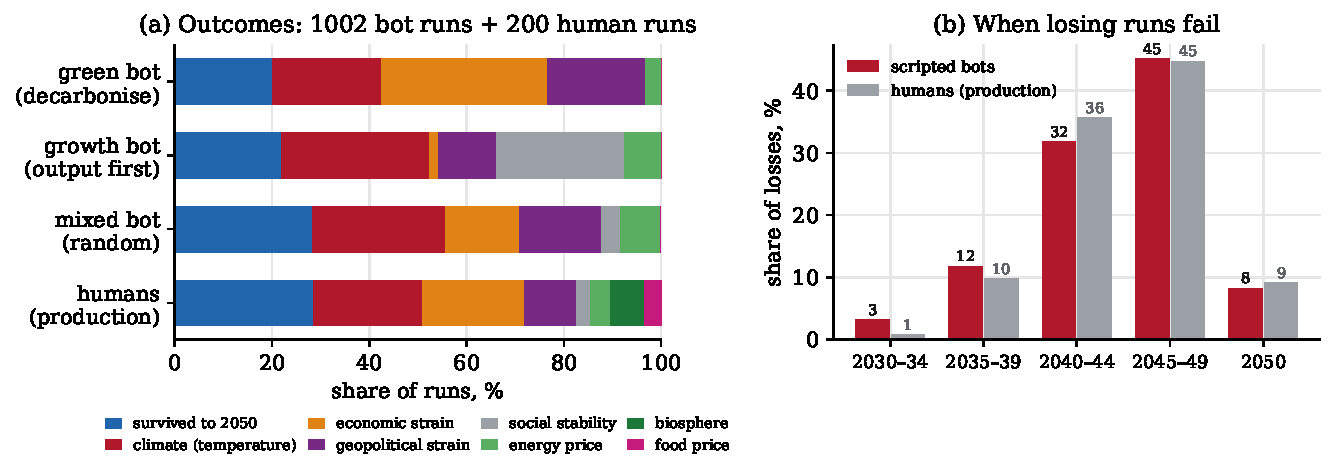
\includegraphics[width=\linewidth]{fig10_game_outcomes.pdf}
\caption{Game-mechanical simulation on the model core ($1{,}002$ automated playthroughs, 2023--2050).
\emph{(a)}~Outcome composition by scripted policy archetype: survival share and loss causes. No
doctrinaire strategy dominates, and each dies of its characteristic cause (green of economic
strain, growth of climate and social stability). \emph{(b)}~Timing of failures: $77\,\%$ of losing
runs fail in 2040--2045, as slow accumulators (temperature, debt, tension) come due.}
\label{fig:game}
\end{figure}

\section{Conclusion}

The model presented here links the economy, climate, natural capital, society, politics, geopolitics,
and culture within a single loop and thereby fills a substantive gap between specialized
single-domain models. Its value for strategic planning, scenario analysis, and risk management lies
not in point forecasting but in the ability to play out scenarios coherently, compare alternative
decisions, express uncertainty correctly through ensembles, and detect weak signals of approaching
structural shifts. The economic and climate blocks are empirically anchored and evaluated in a temporal
hold-out test: emissions and temperature retain positive out-of-sample skill against naive
benchmarks, and the economic fit degrades less than twofold --- confirming the in-sample
metrics are structural rather than artefacts of conditioning; the socio-political and geopolitical blocks, which constitute the model's distinguishing
feature, are validated against a more modest but substantive criterion --- improvement over naive
benchmarks. The economic loop has since been deepened: an explicit money-to-prices transmission (a calibrated
quantity-theory term), an endogenous long-run-growth mechanism (R\&D-stock accumulation à la Jones),
a tested forward-looking-expectations mechanism (left off by default, as its marginal effect proved
unstable), and a data-grounded military-capability index (SIPRI military expenditure as a
CINC-style component, validated against the post-2022 militarization record) have all been added. A game-mechanical layer over the same core (Section~\ref{sec:game}) has proved to be more than an
interface: its outcome distributions behave as a stress test of the coupled dynamics (no
doctrinaire strategy dominates; each dies of its characteristic cause), and balancing it surfaced
--- and led to the repair of --- two structural degeneracies invisible to retrospective
validation. The residual limitations --- the fast-approximation climate block, the
discipline-wide uncertainty of damage estimates, and the intrinsically low predictability of conflict
--- are stated honestly and are not obstacles to applying the model in the modes outlined. \textcolor{green}{However, the model is a tool for exploration, not a substitute for domain-specific expertise or for the judgement of policymakers; its outputs are most informative when used comparatively (scenario vs. baseline) and in conjunction with other lines of evidence.}

\clearpage
\appendix
\section{Key parameters and their identification}
\label{app:params}

Each parameter is specified by a prior distribution; below are the central value, the plausibility
range (roughly the $5$--$95$th percentile of the prior), and the main source. The $33$ key parameters carry
literature-grounded priors (each with a source and rationale); the model's full registry comprises
$287$ parameters with calibration-status tags, most of them expert-set or structural, and is
available in the repository (Section~\ref{sec:repo}).

\begin{table}[h]
\centering
\small
\begin{tabularx}{\linewidth}{@{}lccL@{}}
\toprule
Parameter & Central & Range & Source \\
\midrule
Equilibrium climate sensitivity, $^\circ$C & $3.0$ & $1.5$--$6.0$ & IPCC AR6 WG1 (2021); Otto et al.\ 2013 \\
Surface heat capacity & $8.0$ & $6.0$--$18.0$ & Geoffroy et al.\ 2013 (two-layer EBM) \\
Ocean heat exchange & $1.0$ & $0.4$--$1.3$ & Geoffroy et al.\ 2013 \\
Emissions scale & $0.98$ & $0.90$--$1.05$ & Global Carbon Project 2023 \\
Structural decarbonization rate & $0.016$ & $0.010$--$0.030$ & GCP\,/\,WDI carbon-intensity trend 2000--2023; GIM 2015--2023 backtest \\
Capital share $\alpha$ & $0.30$ & $0.22$--$0.40$ & Penn World Table 10; Gollin 2002 \\
Labor share $\beta$ & $0.60$ & $0.50$--$0.72$ & Penn World Table 10; Gollin 2002 \\
Energy elasticity $\gamma$ & $0.042$ & $0.015$--$0.080$ & 2015--2023 backtest; energy literature \\
Capital--energy substitution $\sigma_{KE}$ & $0.40$ & $0.20$--$0.60$ & van der Werf 2008; Koetse et al.\ 2008 \\
Depreciation rate $\delta$ & $0.05$ & $0.03$--$0.08$ & Penn World Table 8/9 \\
TFP sensitivity to R\&D & $0.30$ & $0.10$--$0.60$ & Calibration to backtest \\
Damage coefficient & $0.0078$ & $0.0015$--$0.025$ & Howard \& Sterner 2017 (productivity-corrected central); DICE-2016R2; Burke et al.\ 2015 \\
Pure rate of time preference $\rho$ & $0.015$ & $0.001$--$0.030$ & DICE-2016R2; Stern 2007 \\
Elasticity of marginal utility $\eta$ & $1.45$ & $1.0$--$2.0$ & DICE-2016R2; Stern 2007 \\
Market demand elasticity & $0.40$ & $0.20$--$0.70$ & Labandeira et al.\ 2017 (meta-analysis) \\
\midrule
\multicolumn{4}{@{}l}{\emph{Social block Section~\ref{sec:uq}}}\\
%(structural assumptions; validated by sign and channel, Section~\ref{sec:uq})}}\\
Tension stress from unemployment & 0.010 & 0.007--0.014 & \text{Burke et al.~2015 (cross-country panel); structural prior} \\
Tension stress from inflation & 0.005 & 0.003--0.007 & \text{Based on Alesina et al.~1992 (inflation and social unrest); prior} \\
Inequality effect on tension & 0.0005 & 0.0003--0.0007 & \text{Adapted from Wilkinson \& Pickett 2009 (inequality and social stress)} \\
Trust-anchor strength & 0.060 & 0.039--0.081 & \text{Calibrated to WGI trust persistence; prior}\\
\bottomrule
\end{tabularx}
\end{table}


%Tension stress from unemployment & $0.010$ & $0.007$--$0.014$ & %Structural assumption (higher unemployment raises discontent) \\
%Tension stress from inflation & $0.005$ & $0.003$--$0.007$ & Structural assumption \\
%Inequality effect on tension & $0.0005$ & $0.0003$--$0.0007$ & Structural assumption \\
%Trust-anchor strength & $0.060$ & $0.039$--$0.081$ & Structural assumption (reversion to equilibrium) \\
%\bottomrule
%\end{tabularx}
%\end{table}

\clearpage
\section{Integration benchmark: where sectoral models stop}
\label{app:benchmark}

The breadth-of-coupling claim (Table~\ref{tab:compare}) is made \emph{computational} here. The
design is literature-anchored rather than an internal ablation: for each of three shocks we take a
published conclusion from a named sectoral model, feed GIM the \emph{same} exogenous shock, and ask
whether GIM \emph{(a)}~reproduces the sectoral first-order effect and \emph{(b)}~surfaces a
cross-sector consequence the sectoral model cannot represent by construction. The unit of comparison
is the \emph{decision-relevant conclusion}, not a headline number: GIM is not claimed to compute
emissions or welfare ``better'' than DICE, but to see a consequence DICE is structurally blind to.
Runs are deterministic (the full $57$-country world, a ten-year horizon, extreme events off, so the
only difference between the baseline and shock arms is the injected shock); each scenario also
reports a dose--response sweep on which the sectoral model's slope is, by construction, zero. The
harness and figures are reproducible from the repository (Section~\ref{sec:repo}).

Two methodological points are stated plainly, as they are part of the result. First, GIM's aggregate
resource-\emph{price} subsystem saturates within one simulated year, so a purely price-mediated shock
does not propagate forward; each shock is therefore injected at its first cross-sector transmission
variable --- precisely the channel a sectoral model lacks (a consumer-price wedge for the carbon tax,
an import-bill and reserve burden for the oil shock, a food-supply gap for the crop shock). Second,
the three spillovers differ in magnitude and shape, and are reported as such rather than uniformly
inflated.

\subsection{Carbon tax (anchor: DICE)}

DICE-2016R \citep{nordhaus2017} finds a welfare-optimal carbon price (about \$31/tCO$_2$ in 2015,
rising) whose only first-order effect is lower emissions; it contains no labour market and no
political economy. Fed the same \$50/tCO$_2$ tax, GIM reproduces the emissions decline (about $5.5\%$
over ten years) and, in addition, raises social tension and lowers government trust as the tax's
pass-through to energy prices feeds inflation and unemployment --- the political-economy channel
behind the reversals of the French carbon and fuel tax (2018) and the Australian carbon price (2014).
As the rate increases, the tension response rises monotonically (Fig.~\ref{fig:bench-carbon}), while
DICE's response on that axis is zero.

\begin{figure}[t]
\centering
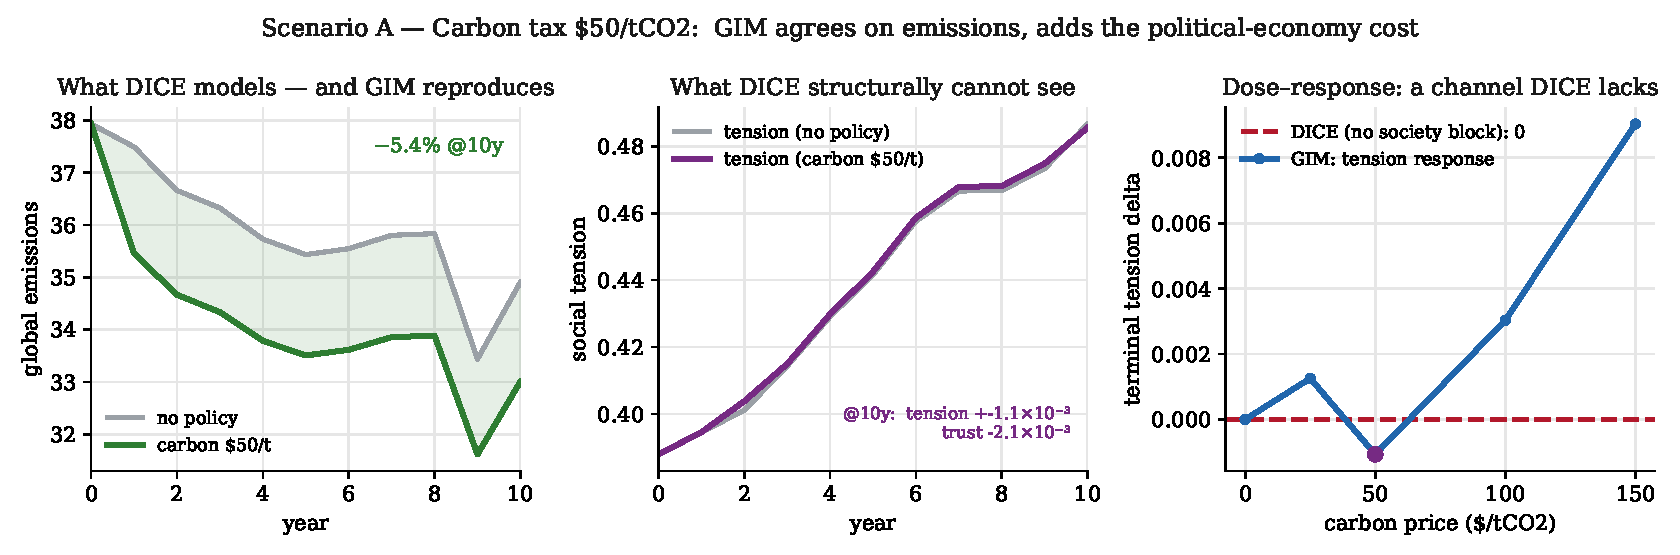
\includegraphics[width=\linewidth]{fig6_integration_carbon.pdf}
\caption{Carbon-tax scenario. Left: GIM reproduces the emissions decline that DICE models. Middle:
GIM adds the social-tension response DICE cannot represent. Right: the response of tension to the tax
rate has a non-zero GIM slope against DICE's zero response.}
\label{fig:bench-carbon}
\end{figure}

\subsection{Oil price shock (anchor: energy-system models)}

An energy-system model such as MESSAGEix resolves an oil-supply shock as a price rise and demand
adjustment, bounded within the energy sector. GIM carries the same shock further, into sovereign
finance: the higher import bill, financed by drawing reserves and issuing debt, brings the most
fiscally fragile importers to their debt-crisis thresholds, and which countries tip is decided by the
model's own debt and interest-rate triggers, not by hand. At a realistic shock (a $20\%$ supply cut,
a burden of about $3\%$ of GDP) the effect is marginal: two additional importers enter crisis. Under a
severe shock (a burden of about $15\%$ of GDP, comparable to the worst historical oil episodes) the
mean importer debt-crisis exposure rises about threefold and four further countries enter sovereign
crisis (Fig.~\ref{fig:bench-oil}). The response is threshold-stepped, and the energy-system model
produces no sovereign crises at any magnitude. This is the mechanism behind episodes such as
Sri Lanka's 2022 default.

\begin{figure}[t]
\centering
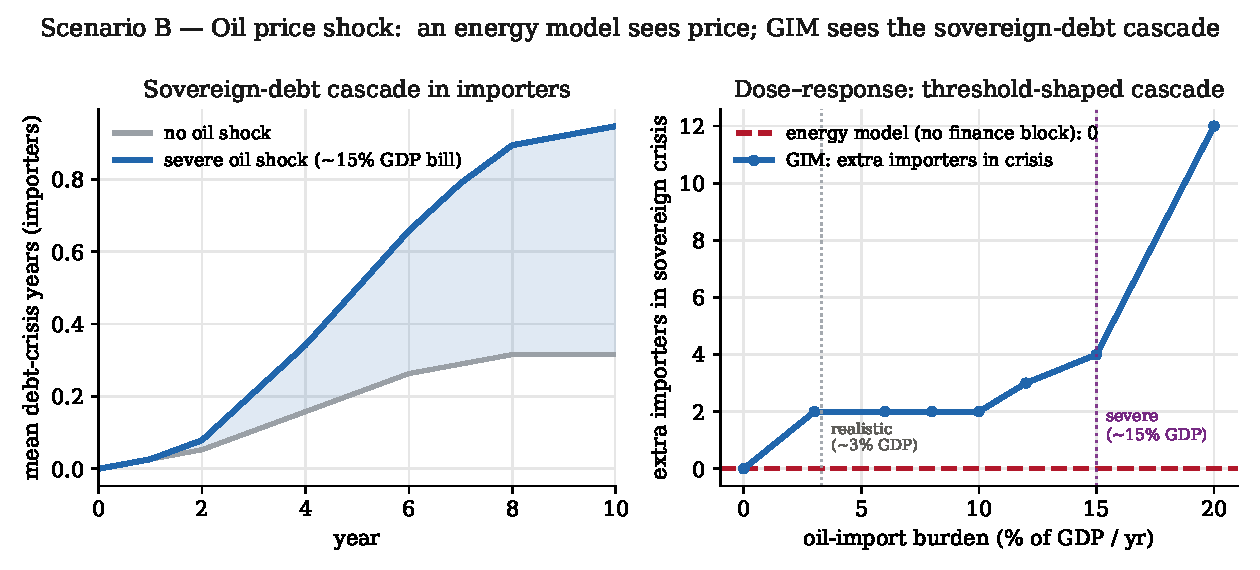
\includegraphics[width=\linewidth]{fig7_integration_oil.pdf}
\caption{Oil-price-shock scenario. Left: importer sovereign-debt-crisis duration under a severe
shock. Right: the response to the import burden is threshold-stepped, marking the marginal
(realistic) and pronounced (severe) points against the energy-system model's zero response.}
\label{fig:bench-oil}
\end{figure}

\subsection{Crop yield shock (anchor: AgMIP and AR6)}

Crop assessments in the AgMIP project and the IPCC Sixth Assessment stop at yield decline and a
food-security index. GIM carries the same yield loss further, into domestic instability: cutting the
production and reserves of the most income-vulnerable importers opens a food-supply gap that raises
protest pressure, and the escalation accelerates as the loss deepens. This is the nonlinear
``crossing into high impact'' documented for food prices and the Arab Spring \citep{lagi2011food}
(a threshold FAO food-price index of $210$). At a severe $50\%$ regional yield loss, food-affordability
stress rises by about $0.11$ and protest pressure by about $0.016$ on the vulnerable subset
(Fig.~\ref{fig:bench-crop}); further along the chain the response attenuates toward regime fragility,
and the endpoint is domestic instability rather than interstate conflict.

\begin{figure}[t]
\centering
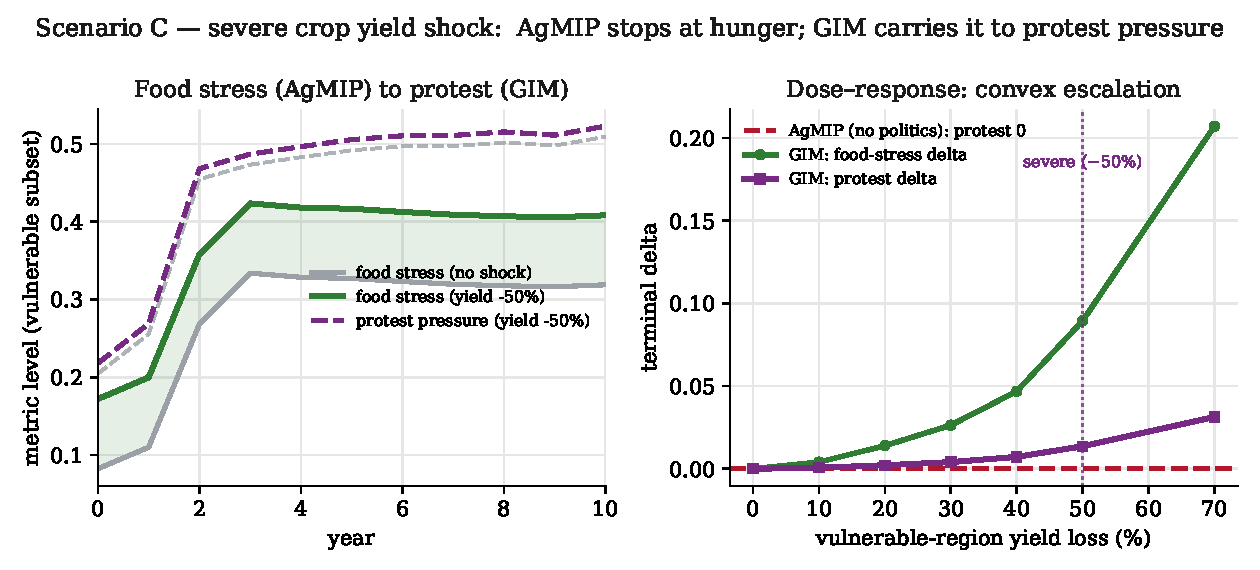
\includegraphics[width=\linewidth]{fig8_integration_crop.pdf}
\caption{Crop-yield-shock scenario. Left: food-affordability stress and protest pressure on the
vulnerable subset. Right: the response to the depth of the yield loss is convex against AgMIP's zero
response on the protest axis.}
\label{fig:bench-crop}
\end{figure}

Across the three channels (Fig.~\ref{fig:bench-summary}) GIM exhibits a positive, measurable slope on
an axis where every sectoral model is, by construction, flat at zero. That gap --- not any single
number --- is the integration dividend, and it is exactly the dimension the coverage table summarizes
qualitatively.

\begin{figure}[t]
\centering
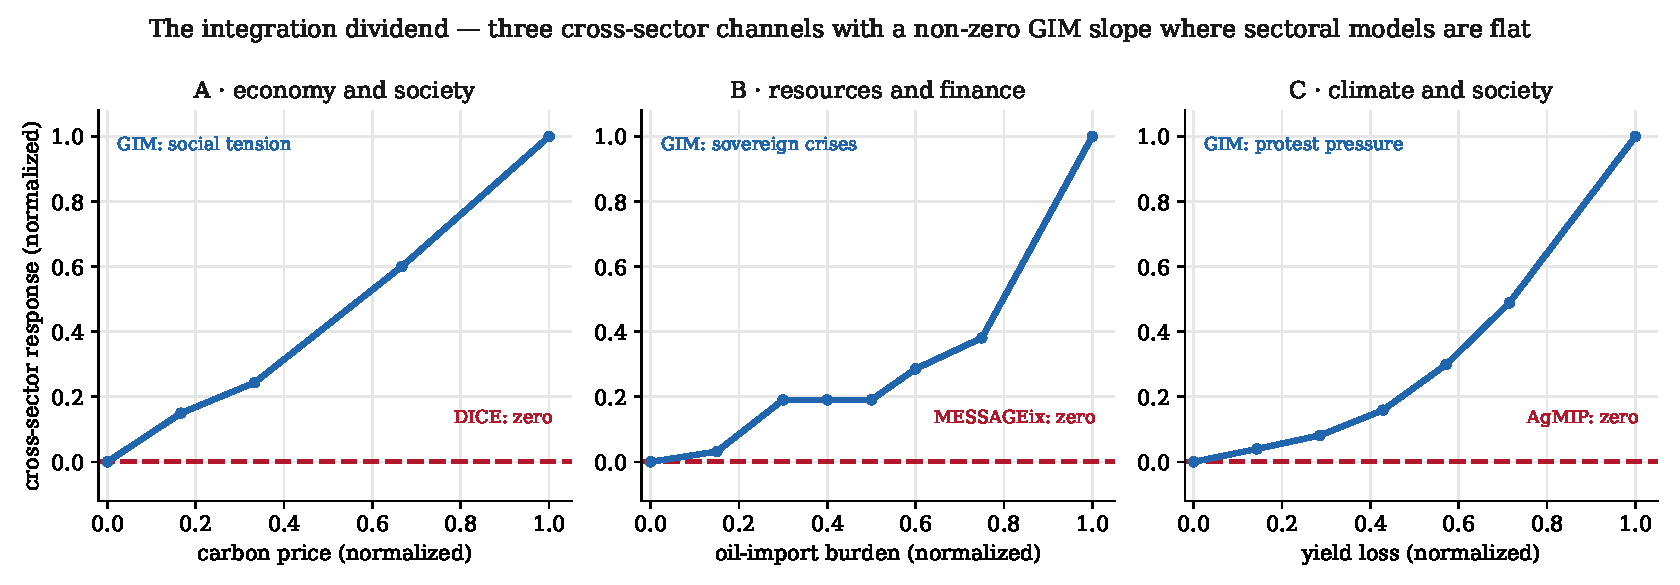
\includegraphics[width=\linewidth]{fig9_integration_summary.pdf}
\caption{The integration dividend. Each panel is one cross-sector channel, normalized to its own
maximum; the dashed line is every sectoral model's zero response on that axis. GIM's slope is smooth
for the economy and society channel, threshold-stepped for the resources and finance channel, and
convex for the climate and society channel.}
\label{fig:bench-summary}
\end{figure}

\clearpage
\bibliographystyle{plainnat}
\bibliography{references}

\end{document}

